\chapter{心脏杂音}

心脏杂音是心脏病的重要体征。心脏杂音可分为收缩期杂音、舒张期杂音、连续性杂音和来往性杂音。收缩期杂音根据杂音开始和终止的时间可命名为全收缩期、收缩中期、收缩早期或收缩晚期杂音。全收缩期杂音与第一心音同时开始,占据全部收缩期。起源于左侧心脏的全收缩期杂音终止于第二心音的主动脉瓣成分,起源于右侧心脏的全收缩期杂音终止于第二心音的肺动脉瓣成分。收缩中期杂音在第一心音之后开始,在第二心音之前终止。起源于心脏左侧的收缩中期杂音终止于第二心音的主动脉瓣成分之前,起源于心脏右侧的收缩中期杂音终止于第二心音的肺动脉瓣成分之前。收缩早期杂音限于收缩早期,与第一心音同时开始,呈递减型减弱,在第二心音之前完全结束,一般在收缩中期或其前结束。收缩晚期杂音在收缩中至晚期开始并延续到第二心音处。

全收缩期杂音以前又称“反流性收缩期杂音”,因为“反流”一词可包括全收缩期的、收缩早期和收缩晚期的杂音,已放弃使用。收缩中期杂音以前又称“喷射性收缩期杂音”,因为收缩中期杂音不一定由于“喷射”所致,所以也应该放弃使用。

全收缩期杂音最常见于二尖瓣关闭不全、三尖瓣关闭不全及室间隔缺损。收缩中期杂音最常见于主动脉瓣狭窄和肺动脉瓣狭窄。收缩早期杂音典型者见于急性重度二尖瓣关闭不全,此外,有三尖瓣关闭不全而右心室收缩压正常时可表现为收缩早期杂音,很小的室间隔缺损杂音也只局限于收缩早期。收缩晚期杂音典型者见于二尖瓣脱垂。

舒张期杂音根据杂音开始的时间可命名为舒张早期、舒张中期和舒张晚期杂音。根据杂音来源于心脏的左侧或右侧,舒张中期杂音随同第二心音主动脉成分或肺动脉瓣成分开始。舒张中期杂音是在第二心音后的一个清楚的周期之后开始。舒张晚期杂音(又称收缩期前杂音)是在舒张晚期开始。舒张早期杂音见于主动脉瓣关闭不全和肺动脉瓣关闭不全。舒张中期杂音主要见于风湿性心脏病二尖瓣狭窄;在没有房室瓣(二尖瓣和三尖瓣)阻塞时,如果流经房室瓣的血容量和血流速度明显增加,造成房室瓣的相对狭窄,也可产生来源于二尖瓣或三尖瓣的舒张中期杂音,例如在重度二尖瓣关闭不全时可产生二尖瓣相对狭窄所致的舒张中期杂音,在重度三尖瓣关闭不全和大的房间隔缺损,可产生三尖瓣相对狭窄所致的舒张中期杂音。舒张晚期或收缩期前杂音见于风湿性二尖瓣狭窄在窦性心律时,因左心房收缩增加导致房室血流增加所致。

连续性杂音指开始于收缩期,并不间断地连续下去,通过第二心音进入全部或部分舒张期的杂音。连续性杂音的最重要特点是杂音通过第二心音而无间断,即收缩期杂音和舒张期杂音连续不间断,而在第一心音前可完全消失。另一特点是杂音在同一听诊部位最响。最熟知的连续性杂音是动脉导管未闭的主、肺动脉沟通,连续性杂音还见于动脉间异常的沟通存在压力阶差、动静脉沟通、颈静脉血流增加引起的颈静脉营营音等。

收缩期和舒张期均可听到杂音,但两期杂音并不连续时,不称为连续性杂音,如室间隔缺损合并主动脉瓣关闭不全、主动脉瓣狭窄合并关闭不全等。这类杂音称为来往性杂音。来往性杂音其收缩期杂音和舒张期杂音最响亮的位置常不在同一部位。

连续性杂音由同一病变引起,来往性杂音由两个不同的病变引起。

心脏听诊发现杂音时,须详细和准确记录其出现的时相(收缩期、舒张期、连续性),持续时限(早期、中期、晚期、全期),音调(高调、中调、低调),强度(Ⅰ~Ⅵ级),音色(吹风样、隆隆样或雷鸣样、喷射样、机器样,乐音样),音质(柔和、粗糙),音形(一贯形、递增型、递减型、菱形),最响的部位,传导方向和位置,以及体位、运动、呼吸和药物对杂音的影响。

听诊结合心音图检查对心脏杂音的判断和提高心脏杂音的听诊能力有极大的帮助。心脏杂音的特点结合心电图、胸部X线片、彩色多普勒超声心动图、心脏核素、CT或核磁显像、心导管检查以及其他检查,能对心脏疾病作出准确的诊断。

根据心杂音出现的部位和期间,对各种心脏病(不包括发绀类先天性心血管病)的鉴别诊断按表\ref{tab15-1}的顺序分别讨论。

\begin{longtable}{c}
 \caption{各听诊区心脏杂音的原因}
 \label{tab15-1}
 \endfirsthead
 \caption[]{各听诊区心脏杂音的原因}
 \endhead
 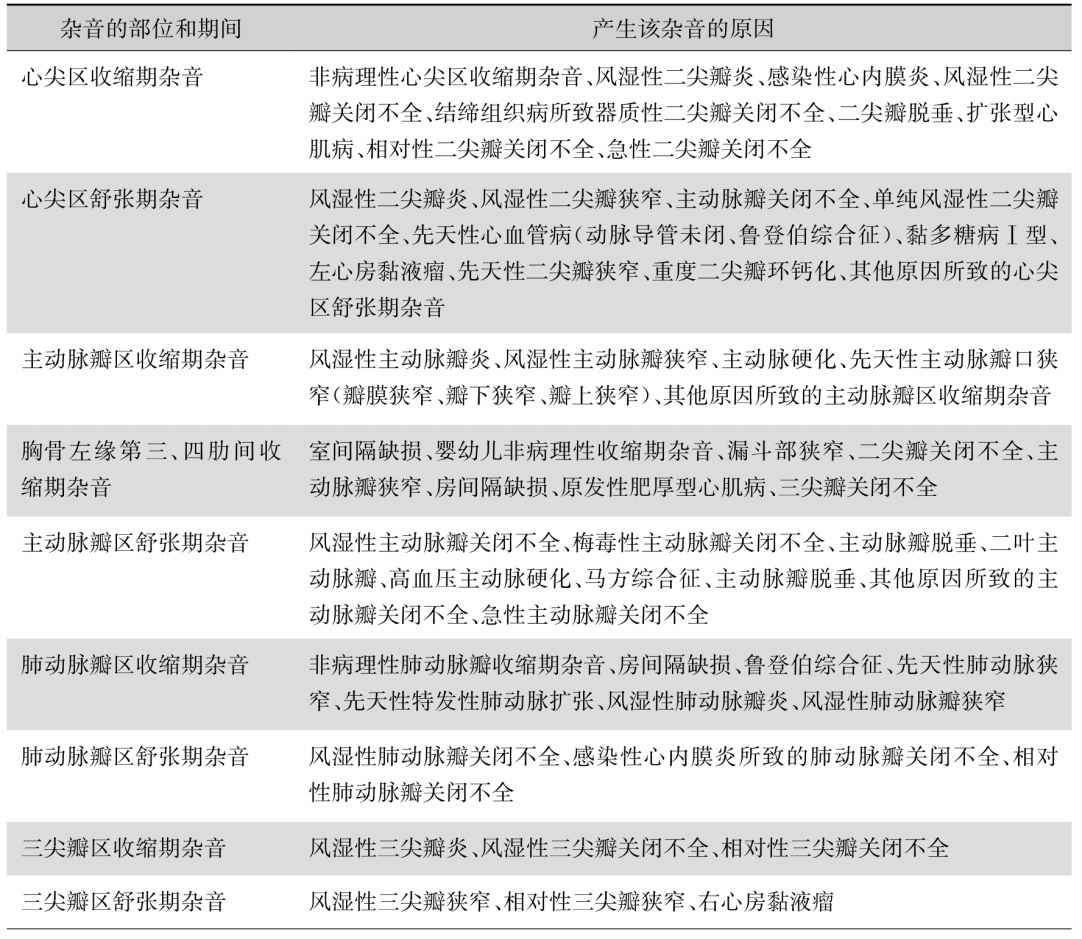
\includegraphics[width=\textwidth,height=\textheight,keepaspectratio]{./images/Image00096.jpg}\\
 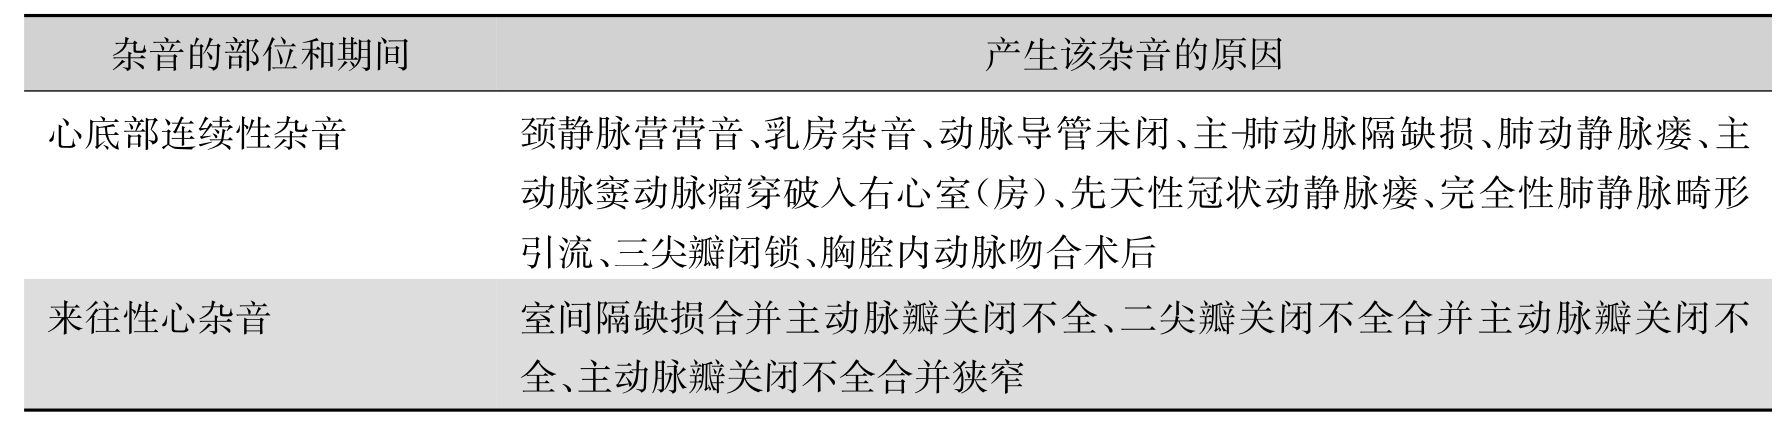
\includegraphics[width=\textwidth,height=\textheight,keepaspectratio]{./images/Image00097.jpg}
 \end{longtable}

心脏听诊还应注意有无心音异常。如第一心音、第二心音有无增强、减弱及分裂,有无病理性第三心音和第四心音,有无其他额外心音如喷射音、喀喇音、开瓣音、心包摩擦音、心包叩击音、肿瘤扑落音、人造瓣膜音等。造成心音异常的原因见表\ref{tab15-2}。

\begin{longtable}{c}
 \caption{异常心音}
 \label{tab15-2}
 \endfirsthead
 \caption[]{异常心音}
 \endhead
 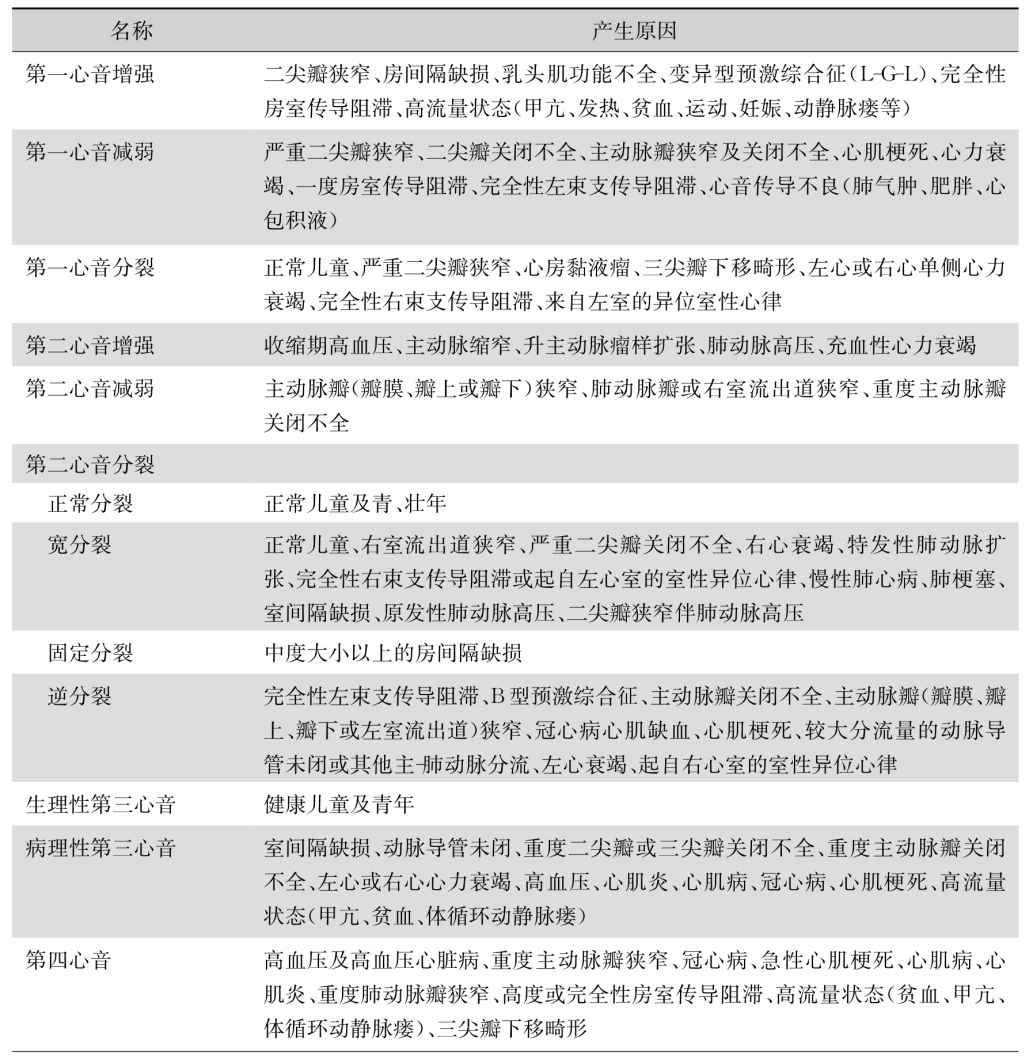
\includegraphics[width=\textwidth,height=\textheight,keepaspectratio]{./images/Image00098.jpg}\\
 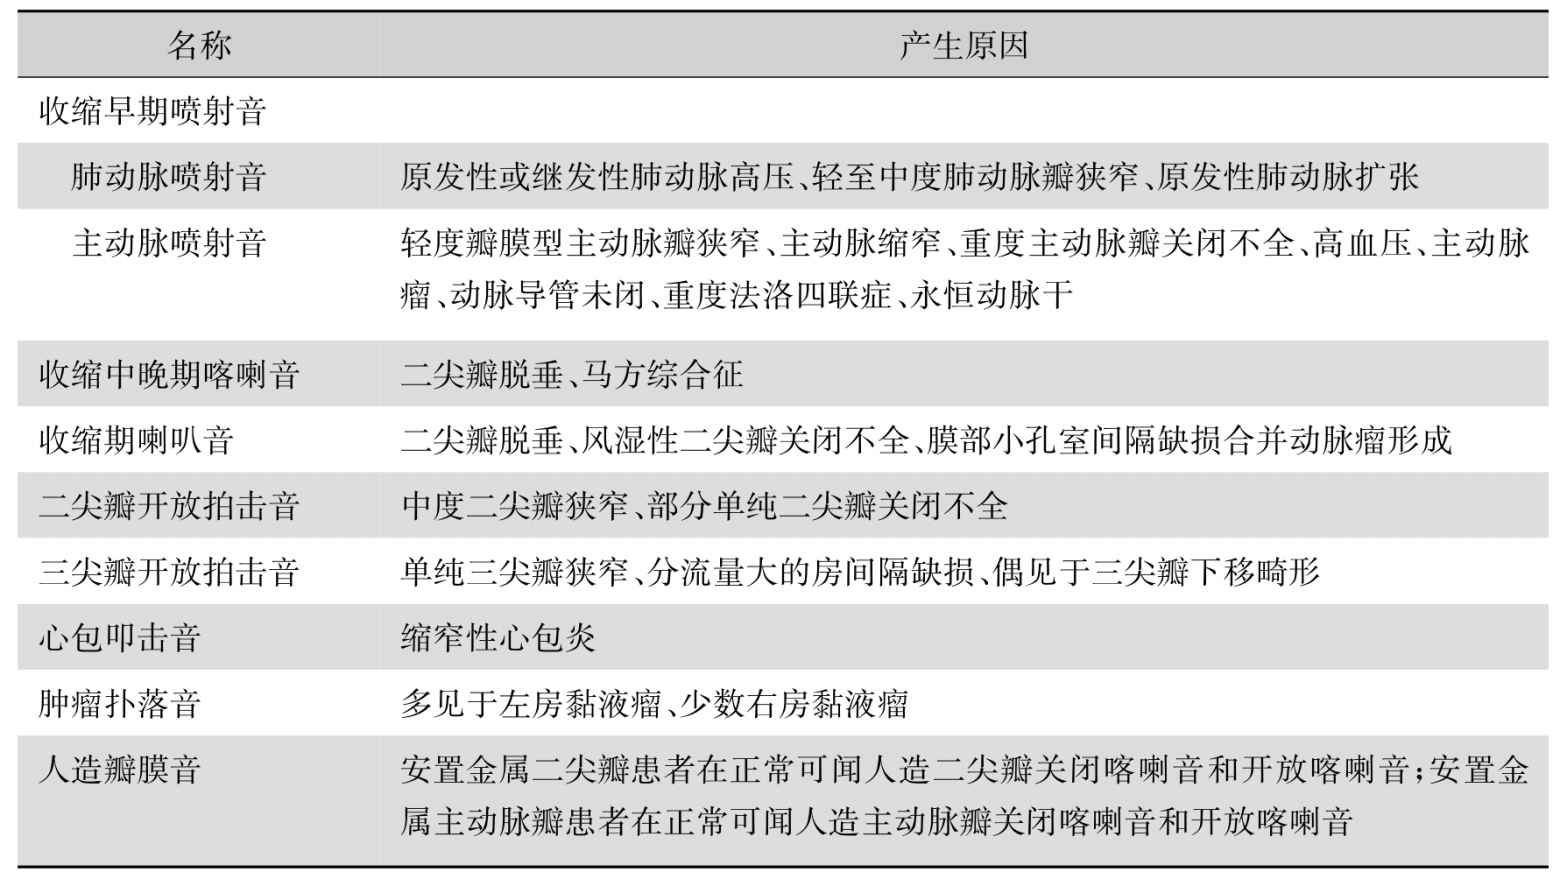
\includegraphics[width=\textwidth,height=\textheight,keepaspectratio]{./images/Image00099.jpg}
 \end{longtable}

\protect\hypertarget{text00124.html}{}{}

\section{45 心尖区杂音}

\subsection{45.1 心尖区收缩期杂音}

\subsubsection{一、非病理性心尖区收缩期杂音}

儿童和青少年多见。心尖区收缩期杂音的响度低(Ⅰ~Ⅱ级)、柔和、吹风样,限于收缩早期或早中期(持续时间不超过收缩期的40\%~60\%),不遮盖第一心音。在心尖区最清晰,局限而不向左腋下传导,运动后杂音减弱或消失,也无心脏增大或心肌炎的征象。

\subsubsection{二、风湿性二尖瓣炎}

风湿性二尖瓣炎是风湿性心内膜炎最常见的表现之一,常引起心尖区收缩期杂音。此杂音是由于二尖瓣风湿性炎症,以及并发心肌炎致二尖瓣环扩张,引起二尖瓣关闭不全所致。常表现为Ⅱ级左右全收缩期吹风样杂音,可向左腋下传导。抗风湿治疗好转后,杂音常消失,少数可发展为慢性二尖瓣病。

\subsubsection{三、感染性心内膜炎}

急性或亚急性心内膜炎均可损坏二尖瓣而引起器质性二尖瓣关闭不全。杂音性质变化是特征性表现之一,一旦出现具有重要诊断价值。当腱索断裂或瓣叶穿孔时可出现新的杂音。

\subsubsection{四、风湿性二尖瓣关闭不全}

二尖瓣关闭不全是临床上较常见的心瓣膜病,早期可呈单纯的风湿性二尖瓣关闭不全,其后常伴发二尖瓣狭窄,两者并存。

如心尖区收缩期杂音占据收缩全期,其响度在Ⅱ级以上,音质比较粗糙,并向腋中线传导,第一心音减弱或被杂音所掩盖,杂音持续存在,并伴有左心房和左心室增大,可确定器质性二尖瓣关闭不全的诊断。早期的器质性二尖瓣关闭不全,可能只有比较响亮的收缩期杂音,尚无左心房与左心室增大的征象,需经较长时期的观察方能确定诊断。

重度二尖瓣关闭不全在心尖部常有响亮的第三心音,是由于左心室迅速充盈所致,也表明患者没有合并严重的二尖瓣狭窄。二尖瓣狭窄较重时,左心室不可能迅速充盈,不能产生第三心音。

单纯重度二尖瓣关闭不全可能伴有舒张中期杂音,是左心室扩大及流经二尖瓣血流量增多,产生相对性二尖瓣狭窄所致。由此产生的舒张中期杂音强度较低而且持续时限较短。第二心音呈宽分裂,因左心射血时间缩短,引起主动脉瓣提早关闭。单纯性二尖瓣关闭不全第一心音从不响亮,也从不延迟。

本病的典型病例通常经由临床与超声心动图检查,便可作出正确的诊断。

器质性二尖瓣关闭不全的收缩期杂音,须与其他原因的收缩期杂音相鉴别:

\paragraph{1.三尖瓣收缩期杂音}

常较近中线,近胸骨下端最响,深吸气末期增强。

\paragraph{2.室间隔缺损杂音}

最响的位置在胸骨左缘第四肋间,不向左腋下传导,比较粗糙,常伴有震颤。

\paragraph{3.非病理性收缩期杂音}

其杂音特点参见上文。这时收缩期杂音是唯一的发现,而无器质性心脏病的证据。其杂音特点参见上文。

\subsubsection{五、结缔组织病所致的器质性二尖瓣关闭不全}

硬皮病病变可累及心内膜与瓣膜,能造成心瓣膜病,累及二尖瓣。系统性红斑狼疮时,炎症可累及心肌与心瓣膜,引起二尖瓣关闭不全较多,而引起二尖瓣狭窄及主动脉瓣关闭不全少见。国内报告一组系统性红斑狼疮100例中,44例心尖区有Ⅱ级以上收缩期吹风样杂音。类风湿关节炎病变可累及二尖瓣、主动脉瓣与三尖瓣,引起关闭不全与狭窄,形成类风湿性心脏病,但以主动脉瓣病变较为多见,此点与风湿性心瓣膜病多侵犯二尖瓣不同。亚当(Ehlers
Danlos)综合征可累及二尖瓣引起关闭不全。本病特点为关节过度伸张,皮肤弹性过强、易脆,常有关节积血、脱位,骨骼和内脏畸形等。病因未明,属常染色体遗传。

\subsubsection{六、二尖瓣脱垂}

二尖瓣脱垂是指乳头肌上的二尖瓣叶脱垂入左心房,以后叶脱垂较多见,双叶脱垂次之,前叶脱垂少见。病因目前认为有冠状动脉硬化性心脏病、风湿性心瓣膜炎、心肌病、马方综合征、Turner综合征、房间隔继发孔缺损、结节性多动脉炎、外伤及瓣膜手术后等。有的病例为家族性,即所谓Barlow病,其二尖瓣特别后瓣呈黏液性变,腱索细长,周围结缔组织松弛,使瓣叶在收缩中晚期脱垂入左房。约30\%病例无明确的病因,称特发性二尖瓣脱垂。

典型体征是收缩期喀喇音及(或)收缩晚期杂音。少数不伴收缩期喀喇音与杂音者称寂静型二尖瓣脱垂。喀喇音多数在收缩中、晚期听到,少数在收缩早期听到,具拍击性,在心尖部或心尖内侧最响。收缩期喀喇音具有易变性的特点,在任何一个时期可以不出现,且可为一个或多个。站立位时喀喇音提早出现且更明显。喀喇音是因松弛的二尖瓣腱索或瓣叶在心脏收缩期突然过度拉紧或翻转而产生,故又名“腱索拍击音”。大多数病例可听到收缩晚期杂音,典型者在一个或更多的中到晚期喀喇音后出现。脱垂严重时为全收缩期杂音,大多为Ⅲ~Ⅳ级,约半数在收缩晚期增强。收缩期杂音是由于二尖瓣叶脱垂入左心房,二尖瓣口不能紧密闭合,致血液反流所引起。少数病例还可听到高频、乐性的“雁鸣音”,并可触及震颤,可能由于二尖瓣叶及腱索在适当的共鸣频率出现震动所致。患者采取坐位时可使收缩期杂音转变为明显的“雁鸣音”。凡使左心室舒张末期容量减少的因素(如深吸气、立位、Valsalva动作屏气期、吸入亚硝酸异戊酯等)可使瓣叶脱垂加重,喀喇音提前,收缩期杂音变长且增强;反之,使左心室舒张末期容量增多的因素(如深呼气、下蹲、解除Valsalva动作舒气期等)可使瓣叶脱垂减轻,喀喇音延迟,收缩期杂音缩短并减轻。

超声心动图是诊断二尖瓣脱垂最有价值的方法。

\subsubsection{七、原发性心肌病}

原发性扩张型心肌病约1/3以上病例出现心尖部收缩期杂音,这是由于心脏明显增大,产生相对性二尖瓣关闭不全所致,须与风湿性二尖瓣关闭不全的杂音相鉴别。本病心脏杂音在心力衰竭期间较响,在心力衰竭控制后即减轻或消失,而风湿性二尖瓣关闭不全时则相反,在心力衰竭期间较弱,而在心力衰竭控制后增强。此外,本病可出现第三心音、第四心音及相对性三尖瓣关闭不全杂音。

原发性肥厚型心肌病时在胸骨左缘下部心尖内侧出现喷射型收缩期杂音。又因常合并二尖瓣关闭不全,在心尖区出现全收缩期杂音。

\subsubsection{八、相对性二尖瓣关闭不全}

高血压性心脏病、贫血性心脏病、主动脉瓣病、冠心病、急性风湿性心肌炎,以及任何原因所致的心肌炎或心肌病,都可引起心脏扩张,并可由下列的原因而导致相对性二尖瓣关闭不全:

1.心肌出现病变时,二尖瓣口纤维环周围的肌肉也显得软弱,致收缩期间瓣膜口未能完全闭合。

2.心脏扩张时,附着于瓣膜的乳头肌与腱索即向下移位,如腱索不能相应地伸长,可妨碍瓣膜口的完全闭合。

相对性二尖瓣关闭不全所致的心尖区收缩期杂音,可根据原发病的存在,病因治疗(如抗贫血、抗风湿)奏效后杂音消失的特点,而与器质性二尖瓣收缩期杂音相区别。

\subsubsection{九、急性二尖瓣关闭不全(腱索断裂、乳头肌功能不全或断裂)}

急性二尖瓣关闭不全的原因主要有二个:瓣膜下二尖瓣装置(腱索或乳头肌)断裂或功能不全;感染性心内膜炎或其他原因所致瓣膜破裂或穿孔。

临床上腱索断裂常见病因有:①在慢性风湿性二尖瓣关闭不全病程中发生;②作为二尖瓣脱垂综合征的合并症,如黏液样变性引起二尖瓣瘤样扩张或破裂、腱索断裂;③胸部钝性或穿透性创伤;④感染性心内膜炎;⑤病因未明的腱索自发性断裂,以后瓣腱索受累较多。

乳头肌功能不全和断裂最常见于冠心病、急性心肌梗死,偶尔可由创伤所致。后内乳头肌血液供应来自右冠状动脉后降支(变异者来自左旋支),血供不及前外侧乳头肌丰富,故下壁心肌梗死时乳头肌功能不全或断裂较多。

急性二尖瓣关闭不全的临床表现与慢性者不同,病情常短期内迅速加重。特别是重度腱索断裂或乳头肌断裂时,大量二尖瓣反流的血液作用于顺应性差而容积未增大的左房,使左房压力短期内上升3~4倍,以致迅速出现左房衰竭性急性肺水肿,之后还可发生右心衰竭。由于心输出量明显减少,患者可出现低血压或心源性休克,如不及时治疗可迅速死亡。

体检心尖搏动有力,但无左室明显扩大的体征,有别于慢性二尖瓣关闭不全。由于主动脉瓣提早关闭,第二心音可有宽分裂,并常有第三心音和第四心音奔马律。房颤少见。急性二尖瓣关闭不全收缩期杂音为非全收缩期,而是收缩早期杂音。该杂音于收缩早至中期呈递减性质,收缩晚期减弱或消失。杂音常是低音调而柔和,很少超过3级。乳头肌功能不全杂音常有以下特点:①杂音多变,即有时杂音较响,有时很轻甚至消失;②不同心动周期中可表现为收缩早期、中期或全收缩期杂音;③心绞痛发作时杂音加强,疼痛缓解后减轻;④过早搏动时杂音较响,而过早搏动后减弱,此点与二尖瓣脱垂相似而有别于其他慢性二尖瓣关闭不全。此外,心尖区第一心音常增强有别于慢性二尖瓣关闭不全的第一心音常减弱。急性心肌梗死所致乳头肌断裂有时杂音很轻但却有严重的肺水肿征,临床上必须加以注意。杂音传导方向取决于前瓣还是后瓣受累,临床上以后瓣受累较常见,反流血流向前,冲击室间隔或主动脉根部,故杂音常在胸骨左缘及心底部最响,并向颈部传导,可误诊为主动脉瓣狭窄或室间隔缺损。若前瓣受累,反流血液流向左房后壁,杂音向左腋下、头部和脊柱传导。

急性二尖瓣关闭不全的特点是心尖区或胸骨左缘(累及后瓣或后内乳头肌断裂)新出现的收缩期杂音或原有杂音加重,伴临床症状的迅速恶化,可出现急性肺水肿征象。心脏不大。心电图有窦性心动过速,可有急性心肌梗死图形而多无左房、左室增大。X线胸片心影无明显增大而有肺水肿征。肺毛压曲线有高大的V波。超声心动图可见腱索或乳头肌断裂,大量二尖瓣反流、二尖瓣呈连枷状改变,左房、左室则无明显增大,是最可靠的诊断手段。

\protect\hypertarget{text00125.html}{}{}

\subsection{45.2 心尖区舒张期杂音}

\subsubsection{一、风湿性二尖瓣炎}

急性风湿性心脏炎患者(大部分为青少年与儿童),在心尖区可出现舒张中期雷鸣样杂音(Carey
Coombs杂音)。此杂音较轻微、柔和、短促,起始部分较响亮,或起始于第三心音之后。其发生机制可能由于瓣膜发炎致其弹性减退,二尖瓣开放受限所致。抗风湿治疗心脏炎痊愈后,此杂音常消失。

\subsubsection{二、风湿性二尖瓣狭窄}

二尖瓣狭窄一般为风湿性,只偶尔为先天性或其他原因所致。国内统计材料风湿性心瓣膜损害95\%~100\%侵及二尖瓣,单纯的二尖瓣病变占70\%~90.9\%。国内成年人慢性风湿性心瓣膜病中,约1/3至半数无明确风湿热病史。风湿性二尖瓣狭窄以女性较为多见。患者往往呈二尖瓣病面容,两颊潮红而口唇发绀,外貌也往往显得较为年轻,对提示诊断有一定的意义。

二尖瓣狭窄与主动脉瓣膜病的临床不同点是较早出现代偿功能不全症状,患者常主诉劳力时甚至安静时出现心悸、气促,此症状对诊断可有重要的提示。有时患者有反复发作的咯血史,也是提供诊断此病的线索。

单纯性二尖瓣狭窄不引起左心室增大,心尖搏动初期也无移位。如右心室增大,心尖可向外侧移位,但不向下移位。如心尖向外向下移位,则非单纯性二尖瓣狭窄,而可能合并二尖瓣关闭不全或主动脉瓣膜病。因此,心尖搏动的视诊与触诊有重要诊断意义。

触诊时可触及心尖区舒张期震颤。心尖区舒张期震颤恒为病理性,且指示二尖瓣狭窄,其他原因所致的心尖区舒张期杂音一般不伴有震颤。如病情发展发生右心室肥厚,心前区呈明显的弥漫性搏动。

风湿性二尖瓣狭窄的听诊特征有以下几点:

\paragraph{1.心尖区第一心音增强}

产生原因是二尖瓣狭窄使左心室充盈时间延长,因而二尖瓣在舒张末期张开较大,且保持在左心室腔中的最低位置,当收缩期左心室内压突然升高,瓣膜关闭血液又突然减速,于是产生较强的第一心音。此外,单纯二尖瓣狭窄左室容量小,振动的物体比较小,因而振动的频率增高,振幅增大。

\paragraph{2.心尖区舒张中期杂音}

二尖瓣狭窄的舒张中期杂音通常局限于心尖区一定部位,范围较狭小,音质粗糙,一般为隆隆样。舒张中期杂音轻的只有Ⅰ级,要使患者取左侧卧位后立即听诊,在最初3~4个心动周期才能听到,有时要在运动后取左侧卧位才能听清楚。杂音响亮者可达Ⅲ~Ⅳ级,并伴有舒张期震颤。但杂音的响度并不提示狭窄的程度,轻到中度狭窄杂音反而很响。极轻度的狭窄可以没有杂音。二尖瓣狭窄舒张期杂音有时因心脏极度顺钟向转位,致使杂音在左腋下部最为清楚,听诊时应予注意。二尖瓣狭窄舒张期杂音为舒张中期杂音,在第二心音一段时间后开始,如有二尖瓣开放拍击音,则在拍击音之后开始。而主动脉瓣与肺动脉瓣的舒张期杂音,则均紧接于第二心音之后,为舒张早期杂音。

二尖瓣狭窄的舒张中期杂音于收缩期前增强(递增型舒张期杂音)具有特征性,此收缩期前增强的杂音为高调吹风样杂音而非隆隆样杂音,易误诊为二尖瓣关闭不全的收缩期杂音。因这一递增型舒张期杂音是由于心房强力收缩所产生,当晚期病例有高度心房扩大、心房收缩力减弱,或发生心房颤动时,则此杂音不出现。

如由于二尖瓣狭窄而继发肺动脉高压,可出现相对性肺动脉瓣关闭不全,在肺动脉瓣区听到舒张早期高调哈气样递减型杂音,一般较轻柔,称史氏(Graham
Steell)杂音,此杂音也可传至心尖区。

心尖区舒张期杂音的鉴别诊断,必须参照其他特征性体征。如兼有第一心音增强与二尖瓣开放拍击音的存在,则可肯定为器质性二尖瓣狭窄(左心房黏液瘤可为例外)。如舒张期杂音起源于主动脉瓣关闭不全(Austin
Flint杂音),则应同时有主动脉瓣区舒张期杂音与周围血管征,且无左心房增大。由主动脉瓣或肺动脉瓣关闭不全传导至心尖区的舒张早期杂音,常为柔和的吹风样,而非隆隆样,且为递减型,不表现为递增型。

临床上,有两种情况可能在二尖瓣狭窄病程中舒张期杂音很轻或听不到,一种情况是因狭窄很轻,第二种情况是极度狭窄或伴有心力衰竭存在(“哑型”二尖瓣狭窄)。这些病例必须结合全面的检查及超声心动图检查结果才能作出诊断。

\paragraph{3.二尖瓣开放拍击音}

此音是诊断二尖瓣狭窄的重要体征之一。在单纯性二尖瓣狭窄有此体征者达83.8\%。在少数的二尖瓣狭窄合并关闭不全的病例也可有此体征。此音在胸骨左缘稍外第四肋间最响,紧随第二心音,但又与第二心音之间有一明显的距离。这是一种响亮、清脆而具有拍击样的声音。在下列情况下可使此音更加清楚:①坐位时多数比卧位时清楚;②仰卧位高举两下肢比平卧清楚;③深呼气状态多能使此音加强。

如有瓣膜钙化、肺血管阻力显著升高、主动脉瓣关闭不全伴有二尖瓣病、重度二尖瓣关闭不全时,二尖瓣开放拍击音常消失。一般而言,此音距第二心音的距离越短,瓣膜狭窄的程度越严重。

二尖瓣开放拍击音应与第三心音及第二心音分裂相区别。第三心音的音调较低,无拍击性质,在心尖区最响,且与第一心音和第二心音的时间距离比较均匀。第三心音极少见于二尖瓣狭窄,而常见于二尖瓣关闭不全,因此音的形成是由于左心室迅速充盈而产生震动所致,而二尖瓣狭窄时左心室不可能迅速充盈。第二心音分裂则在肺动脉瓣区最清楚,此分裂的两个声音的距离极短,平均为0.04秒,在深吸气时常较清楚。

\paragraph{4.肺动脉瓣区第二音增强}

二尖瓣狭窄时出现此体征表示有肺淤血。肺动脉瓣区第二音增强不出现于早期的二尖瓣狭窄;晚期病例当合并相对性三尖瓣关闭不全与肝大时肺动脉瓣区第二音也不增强。二尖瓣狭窄合并相对性三尖瓣关闭不全的诊断根据是:胸骨左缘与心尖区之间收缩期杂音、颈静脉搏动、收缩晚期肝脏扩张性搏动,以及高度的右心房增大。

二尖瓣狭窄的心脏形状与病情轻重有关。在早期病例,心脏大小可正常,形状也可正常。稍晚期则由于左心房增大,而形成大小正常的二尖瓣型心脏。晚期则形成增大的二尖瓣型心脏。二尖瓣型心脏的形成是由于心腰隐没所致,其原因是由于左心房增大、肺动脉段扩张,以及右心室肥厚与扩张所致的心脏转位。

X线检查对单纯性二尖瓣狭窄的诊断相当可靠。但需注意,少数无心脏病变的人也可出现轻度甚至较为明显的食管压迹移位;另一方面,临床上也有少数二尖瓣狭窄早期病例以及联合瓣膜损害,无左心房增大的X线征象。超声心动图检查对诊断二尖瓣狭窄有重要价值。

心电图早期无改变,较晚期出现右心室肥厚、电轴右移与二尖瓣型P波。心房颤动也常见。

哑型二尖瓣狭窄少见,临床提示哑型二尖瓣狭窄的表现为:风湿热病史,胸骨左缘或剑突下右室搏动有力,肺动脉瓣第二心音亢进,二尖瓣开瓣音,心尖第一心音亢进,心电图示二尖瓣型P波及右室肥厚,X线显示左房增大和肺动脉高压等。当患者有上述表现时,即使无舒张期杂音,也应注意哑型二尖瓣狭窄的可能性。超声心动图可明确诊断。

\subsubsection{三、主动脉瓣关闭不全}

在严重的单纯性主动脉瓣关闭不全病例,有时可在心尖区听到低音调的隆隆样舒张期杂音,收缩期前增强,称为弗氏(Austin
Flint)杂音。此杂音是一种功能性杂音,它不在代偿功能良好的主动脉瓣关闭不全中出现,而仅在左心室衰竭的情况下出现,且在代偿功能恢复时又重新消失。弗氏杂音的发生机制是:当主动脉瓣关闭不全心脏舒张时,大量血液从主动脉反流入左心室,将二尖瓣的前瓣冲起,造成相对性二尖瓣狭窄。弗氏杂音与器质性二尖瓣狭窄舒张期杂音有时不易鉴别,鉴别要点为:①弗氏杂音较为柔和,多不伴有震颤;②不伴有二尖瓣开放拍击音与心尖区第一心音增强;③不伴有明显的左心房增大;④心电图显示左心室肥厚,而无右心室肥厚与二尖瓣型P波。

\subsubsection{四、单纯风湿性二尖瓣关闭不全}

本病有时可在心尖区出现舒张中期隆隆样杂音。此杂音持续时间较短(0.12~0.25秒),一般不伴有收缩期前增强,杂音的起始部分多较响亮,或开始于响亮的第三心音之后。杂音强度有时可达Ⅵ级,易误诊为二尖瓣狭窄合并关闭不全。此杂音的产生是由于心脏收缩时,大量血液从二尖瓣口反流入左房,于舒张期又再度流入左室,使舒张期通过二尖瓣口的血流量明显增多所致。但在单纯二尖瓣关闭不全时,心尖区第一音减弱,且左心室增大,不符合二尖瓣狭窄的诊断。

\subsubsection{五、先天性心血管病}

动脉导管未闭可在心尖区出现短促低调的舒张期杂音。杂音产生的机制主要是由于伴有大量左至右的分流,通过二尖瓣的血流量增多,致在左心室快速充盈期产生一低音调而短促的非递增型舒张中期杂音。鲁登伯(Lutembacher)综合征的病理改变是房间隔缺损伴二尖瓣狭窄。此时出现的心尖区隆隆样舒张期杂音,乃由于先天性二尖瓣狭窄所致。

\subsubsection{六、黏多糖病Ⅰ型}

黏多糖病Ⅰ型又称承霤病(gargoylism),也称Hurler综合征和怪面病,主要见于小儿,病因与酸性黏多糖代谢紊乱有关。患者有特殊的承霤病样面容:两颞和额部突出、马鞍鼻、大鼻孔、眼裂小、口唇厚、下颌短小等,并有身材矮胖、智力障碍、角膜混浊、听力障碍、心血管或呼吸道病变、爪状手、肝脾大等表现。此病70\%以上并发心血管病变,心肌内结缔组织细胞肿胀、肥大与空泡形成,心瓣膜有结节形成与增厚;病变好侵犯二尖瓣,可出现心尖区收缩期与舒张期杂音。X线检查显示心脏普遍性增大,但无特征性心电图改变。2/3承霤病患者因心力衰竭而死亡,死亡年龄平均11岁。患者尿中含有大量酸性黏多糖(AMPS),此种物质的测定对诊断有重要意义。

\subsubsection{七、左心房黏液瘤}

有蒂的左心房黏液瘤,其临床表现往往酷似二尖瓣狭窄,包括心尖区第一心音亢进与隆隆样舒张中期及收缩期前杂音。二尖瓣口发生显著的血流障碍时,可产生阵发性呼吸困难、心悸、晕厥等症状。

患者有下列情况时提示左心房黏液瘤的可能性:①并非由于体力活动所致的心悸、呼吸困难、咯血、交替性低血压、眩晕、急性心源性脑缺血综合征发作与间歇性发热;②出现动脉性微小栓塞所致的周围性疼痛点,而无感染性心内膜炎或二尖瓣膜病的证据;③应用强心剂治疗不能改善的肺淤血;④听诊与X线检查所见类似二尖瓣狭窄合并关闭不全;⑤体位改变或长期观察时发现心杂音改变;⑥约1/3患者可听到舒张早期肿瘤扑落音。

X线检查显示左心房增大。超声心动图诊断价值甚大,显示左心房内有异常迅速移动的反射光团。超声心动图还有助于黏液瘤与巨大球形血栓形成相鉴别。左心房黏液瘤有随心动周期迅速移动的特征,而血栓则无;黏液瘤大多位于心房中隔,而血栓大多位于心房后壁。

\subsubsection{八、先天性二尖瓣狭窄}

极少见,二尖瓣呈特征性降落伞状畸形,与风湿性二尖瓣狭窄有类似症状、体征,但在幼儿期出现。

\subsubsection{九、重度二尖瓣环钙化}

重度二尖瓣环钙化属老年退行性心瓣膜病。严重二尖瓣环钙化可致二尖瓣基底部增厚、硬化,瓣叶正常活动受限,除产生二尖瓣狭窄外,部分可伴有功能性二尖瓣关闭不全。超声心动图示二尖瓣环前后缘呈强回声团块。

\subsubsection{十、其他原因所致的心尖区舒张期杂音}

主动脉瓣狭窄、贫血性心脏病、慢性缩窄性心包炎、高血压动脉硬化、甲状腺功能亢进性心脏病、完全性房室传导阻滞、心肌病、心内膜纤维性变、右室条状附壁血栓等情况,偶亦引起心尖区舒张期杂音,但通常不难与二尖瓣狭窄鉴别。

\protect\hypertarget{text00126.html}{}{}

\section{46 主动脉瓣区杂音}

\subsection{46.1 主动脉瓣区收缩期杂音}

主动脉瓣区收缩期杂音通常为器质性,有时也为功能性。器质性收缩期杂音很多时候伴有收缩期震颤。

\subsubsection{一、风湿性主动脉瓣炎}

风湿性主动脉瓣炎是风湿性心脏炎的部分表现。如风湿性心脏炎患者在主动脉瓣区出现收缩期杂音,可认为存在主动脉瓣炎。如杂音经抗风湿治疗后消失,或以后发展为慢性风湿性主动脉瓣病,即可证实曾患过急性风湿性主动脉瓣炎。

\subsubsection{二、风湿性主动脉瓣狭窄}

风湿性主动脉瓣狭窄男性多于女性。常见的症状是呼吸困难和左心衰竭。有时右心衰竭出现在左心衰竭之前,是因肥厚的室间隔向右侧膨出,侵占右心室腔,引起右心室流出道狭窄所致。

晕厥和心绞痛是突出的症状。晕厥可能导致突然死亡。

严重病例的动脉脉波幅度低、高原形(脉波上升与下降均缓慢);如合并主动脉瓣关闭不全,脉搏呈重波脉;颈动脉搏动减弱,如主动脉瓣狭窄严重,可能观察不到。血压不定,严重病例血压低。由于左心室肥厚,心尖呈抬举性搏动。听诊可听到收缩中期杂音,在主动脉瓣区最响。杂音常响亮,伴有收缩期震颤,并向右颈动脉传导。在很少见的情况下,收缩期杂音在心尖区最响。如心尖区收缩期杂音向左腋窝和左肩胛部传导,则不是主动脉瓣收缩期杂音。杂音清晰地在第一心音之后开始,在主动脉瓣关闭之前终止,而限于收缩中期。杂音的响度和狭窄的程度无密切的关系。当主动脉瓣狭窄极为严重时,收缩期杂音可能显得较短且较柔和。如并发心力衰竭,杂音可能完全消失。

如无严重狭窄,可能听到收缩期喷射附加音。第二心音常呈单音,因第二心音的主动脉瓣成分延迟而置于肺动脉瓣成分之上。有时主动脉瓣区第二心音消失,提示瓣膜严重钙化,致主动脉瓣成分消失。可能出现奔马律。后期出现相对性二尖瓣关闭不全。虽然收缩中期杂音是主动脉瓣狭窄的最早体征,但主动脉瓣狭窄患者中10\%无此杂音。

心电图常显示左心室肥厚。成人心电图改变的严重性与狭窄的程度成正比,但儿童中严重主动脉瓣狭窄者的心电图可以正常。有时有深的Q波酷似心肌梗死。偶有左束支传导阻滞或房室传导阻滞,特别是当有心力衰竭时。

X线检查示左心室边缘圆钝和突出,可见瓣膜钙化;可有狭窄后主动脉扩张,但不如先天性主动脉瓣狭窄常见。左心房可能轻度增大。左心室造影显示僵硬的圆顶形主动脉瓣膜和实际上固定的瓣膜口。

心导管检查显示左心室收缩压升高,左心室和主动脉之间的压力阶差因病例而不同,从数mmHg至200mmHg以上。压力阶差在50mmHg或以上时,提示有外科治疗的需要。如发生心力衰竭,心输出量降低,压力阶差可能显现低的假象。左心房压力曲线可能有大a波。主动脉压力曲线显示很慢的升支和低而显著的升支切迹。主动脉瓣狭窄的程度越严重,升支上的切迹越低。主动脉平均血压低。

超声心动图可显示主动脉瓣狭窄的程度和狭窄前后的压力阶差。

\subsubsection{三、先天性主动脉口狭窄}

先天性主动脉口狭窄约占先天性心脏病的5\%,按病变部位可分为三种类型:①主动脉瓣膜狭窄;②主动脉瓣下狭窄;③主动脉瓣上狭窄。

\paragraph{1.先天性主动脉瓣膜狭窄}

此型最为常见。病理上二叶主动脉瓣畸形最多,占70\%。融合的左、右冠瓣叶与无冠瓣叶之间仅留下狭小的瓣孔。有的病例主动脉瓣仅有一个瓣叶,呈隔膜状,狭小的瓣孔位于瓣膜的中央或偏向一侧。

听诊可闻收缩中期杂音。杂音起于收缩期喷射音或第一心音之后,止于第二心音主动脉瓣成分之前,在胸骨右缘第一、二肋间最响,响度一般为Ⅲ~Ⅳ级,多伴有震颤。杂音向胸骨上窝及沿颈动脉传导,亦向胸骨左缘及心尖部传导。杂音的强度和狭窄的程度不成正比,这点不同于肺动脉瓣狭窄。但轻度狭窄的杂音一般较轻,发生心衰时杂音亦减弱。

在心尖部和胸骨左缘有时可闻喷射性的乐音样杂音,是狭窄的瓣膜震动所产生,其强度一般不如胸骨右缘的杂音响亮。

第二心音主动脉瓣成分正常或增强,严重狭窄者可减弱。第二心音呈正常分裂时,表示狭窄为轻度。重度主动脉瓣狭窄时,第二心音呈反常分裂。

常有收缩早期高调喷射音,在胸骨右缘第二肋间或心尖部最响。喷射音的存在是先天性主动脉瓣膜狭窄的听诊特征之一,在鉴别诊断上有重要意义。

第三心音常出现于儿童或左心衰竭的患者。严重狭窄的病例多出现第四心音。此外,约1/8~1/5的病例可听到Ⅰ~Ⅱ级柔和的主动脉瓣关闭不全舒张早期杂音。

儿童期多无特殊症状,青少年时期才逐渐出现明显的呼吸困难、晕厥和胸痛。

轻度主动脉瓣膜狭窄心电图可正常,中、重度患者可出现左心室肥厚、劳损。

胸部X线平片轻症患者心影大小可正常,严重患者左心室增大,可见升主动脉狭窄后扩张。

超声心动图检查可见主动脉瓣膜开放受限,呈单瓣、双瓣或四瓣畸形。

左心导管检查可测定主动脉瓣两侧压力阶差。左室造影可确定狭窄部位、解剖形状及狭窄程度。

\paragraph{2.主动脉瓣下狭窄}

此型在先天性主动脉口狭窄中约占9\%,狭窄病变位于主动脉瓣环的下方,又分为三型:①孤立性主动脉瓣下狭窄;②主动脉瓣下管状狭窄;③特发性肥厚性主动脉瓣下狭窄。

先天性孤立性主动脉瓣下狭窄是在左心室流出道有一纤维环,其中央仅有小孔造成左心室血流通道狭窄。此型临床症状、听诊与先天性瓣膜狭窄极相似,但听诊上有两点不同:除个别外,绝大多数无收缩早期喷射音;第二心音的主动脉瓣成分正常或减弱。超声心动图及左心导管检查可确定诊断。

先天性主动脉瓣下管状狭窄是在左室流出道有肌肉纤维的管状狭窄,极少见。其症状与先天性主动脉瓣膜部狭窄相似,但收缩中期杂音在胸骨左缘第二至第四肋间最响,Ⅲ~Ⅳ级,粗糙,不少病例可在胸骨左缘第三肋间听到Ⅰ~Ⅲ级舒张早期递减性杂音,个别病例可听到收缩早期喷射音,少数病例有第三心音和第四心音。

特发性主动脉瓣下肥厚狭窄实际上应称为原发性肥厚型心肌病,较多见,其收缩期喷射性杂音于胸骨左缘下部最响,将在此节专门叙述。

\paragraph{3.主动脉瓣上狭窄}

此型极少见,通常是紧接主动脉窦之上有一局限的节段性狭窄,狭窄后的主动脉正常或缩小。此外,可有纤维隔膜状狭窄或升主动脉普遍性狭窄。

约1/3患者有家族史,男性发病较多。患者多有特殊面容:前额宽、颊呈袋状、两眼距离宽、内眦赘皮、鼻翼上翻、宽嘴唇、尖下巴、牙齿错位咬合、声音低而带金属样、智力发育迟滞等。右侧肱动脉压常高于左侧20mmHg以上,并常有高钙血症。

听诊粗糙响亮的喷射性收缩期杂音在胸骨右缘第一肋间或胸骨上窝最响,并向右侧颈部传导。第二心音主动脉瓣成分正常或减弱,无喷射音,可以有主动脉瓣舒张早期杂音,但不常见。

心电图常有显著的ST段和T波改变。X线检查左心室常中度增大,但无狭窄后升主动脉扩张,主动脉弓部小或消失。超声心动图检查常只能发现接近主动脉瓣部位的升主动脉管腔狭窄或异常回声。左室造影检查可确定狭窄部位、程度及解剖形状。

\subsubsection{四、主动脉硬化}

主动脉硬化在老年人,主动脉瓣环发生硬化,硬化性变可蔓延至主动脉瓣,并产生收缩期杂音。此型主动脉瓣狭窄临床意义甚少,只发生于老年人,与风湿性者发病年龄不同,其响度也较弱,音质也无后者的粗糙与搔抓样。

\subsubsection{五、其他原因所致的主动脉瓣区收缩期杂音}

梅毒性主动脉瓣关闭不全、升主动脉扩张(如主动脉缩窄)、继发性高动力性综合征(如脚气病性心脏病及甲状腺功能亢进性心脏病)等,也可引起主动脉瓣区收缩期杂音,通常临床意义甚少。

\protect\hypertarget{text00127.html}{}{}

\subsection{46.2 胸骨左缘第三、四肋间收缩期杂音}

\subsubsection{一、室间隔缺损}

右心室内腔是一条由右室流入道与右室流出道(动脉圆锥)所构成的管道。此两者所构成的角有一条厚的肌性嵴,称为室上嵴。此嵴是动脉圆锥与右心室的其余部分的分界。

室间隔缺损一般按解剖部位分为嵴上型、嵴下型、隔膜后型和肌型。

1.嵴上型
不常见,缺损很高,直接在主动脉瓣和肺动脉瓣之下,主动脉瓣环可能因缺乏支持致瓣叶脱垂,引起主动脉瓣关闭不全。

2.嵴下型
直接在嵴下和三尖瓣之下,在室间隔的膜部,是最常见的类型。从左心室观察,缺损位于主动脉瓣环之下。

3.隔膜后型 传统上又称房室通道缺损。缺损位置较低,更靠后。

4.肌部缺损 此型最少见,缺损更低,在间隔肌部,最常见的是近心尖部。

室间隔缺损的严重程度,在临床上可区分为以下三种:

1.小至中等的缺损
肺动脉血流量和压力以及肺血管阻力正常或接近正常。缺损小、分流量小的病例,相当于以往所称的Roger病,一般无症状。

2.严重的缺损
肺动脉压力和肺血管阻力升高,但未达到体动脉的水平,因此不出现发绀。

3.艾森曼格(Eisenmenger)综合征 缺损直径≥2cm,出现右向左分流,出现发绀。

小的甚至中等度的室间隔缺损无发绀,且常无症状。如分流量很大,则出现左至右分流的常见症状,即呼吸困难、反复发作的支气管炎和发育停滞。婴儿时期可发生心力衰竭,多数于1岁内死亡。小的缺损较易并发亚急性感染性心内膜炎。大的缺损常引起心前区隆起,心脏搏动弥散。听诊在胸骨左缘第三、四肋间闻及响亮粗糙的全收缩期杂音,向心前区广泛传导,有时颈部、背部亦可听到。杂音最响处可触及震颤。但如缺损很小,则杂音柔和可呈喷射性。当缺损在间隔的肌部时,杂音最强的位置可能在心尖区。嵴上型缺损的杂音近肺动脉瓣区。呼气时杂音增强。约半数患者因通过二尖瓣的血流量增加,在心尖区有舒张中期杂音,表示肺血流量超过体血流量的2倍。如分流方向相反,此杂音即消失。但须注意不少先天性二尖瓣畸形与室间隔缺损并存,可以引起相同的舒张中期杂音。因左心室充盈迅速,常有响亮的第三心音。在小的缺损时,第二心音的响度正常,第二心音宽分裂。如有肺动脉高压,则第二心音的肺动脉瓣成分增强,出现较早,因而心音分裂的距离变窄,第二心音甚至可以变成单一。如已发生漏斗部肥厚,则第二心音肺动脉瓣成分减弱(或听不到)和延迟。如肺动脉高压显著,则出现肺动脉瓣关闭不全的递减型舒张早期杂音。分流量大时周围动脉的搏动减弱。

心电图:小的室间隔缺损的心电图正常。较大的室间隔缺损显示左心室舒张期容量负荷过重,左心室导联的R波高、Q波深、T波直立。如分流量较大和肺血管阻力升高,可以出现右心室肥厚心电图。完全性或不完全性右束支传导阻滞也可以出现。

X线检查:小的室间隔缺损,其心影正常;中度以上缺损心影增大,肺动脉圆锥突出,可见肺动脉的扩张和搏动,肺血流量增多,左心房增大,两心室增大,主动脉结缩小。当发展到肺动脉高压时,心脏增大以右室为主,肺动脉圆锥及肺门血管影显著扩张。

超声心动图:可显示左房、左室内径增大,伴肺动脉高压时右室、右室流出道和肺动脉也有增宽。二维超声显像可直接看到室间隔回声中断。彩色多普勒检查可估计缺损部位、大小及分流方向。

心导管检查与选择性心血管造影右心室血氧含量较右心房高出0.9容积\%以上或平均血氧饱和度高出3\%以上,据此作出心室水平左至右分流的诊断。但必须除外右心室血氧含量增高的其他原因,例如:①动脉导管未闭或主-肺动脉隔缺损合并肺动脉瓣关闭不全;②主动脉窦动脉瘤穿破入右心室。当分流量小时,右心室的血氧饱和度可以正常,可用指示剂方法以证明分流。小至中等度的室间隔缺损,其右心室和肺动脉的压力以及肺血管阻力正常或只轻度升高。严重的室间隔缺损时可见:①右心室和肺动脉压力升高,但低于左心室的压力;②肺血流量和肺血管阻力增加;③除非有心力衰竭或合并三尖瓣畸形,肺毛细血管嵌入压正常或轻微升高。

左心造影从左前斜位观察,可见从左心室注入的造影剂进入右心室。注入造影剂于右心室中,对除外其他先天性畸形如矫正型大血管错位(corrected
transposition)等,有极大的诊断价值。

\subsubsection{二、婴幼儿非病理性收缩期杂音}

婴幼儿时期在胸骨左缘通常有非病理性收缩期杂音,呈喷射型,但不伴有震颤。儿童长大后此杂音便消失,其中少数无疑是小的室间隔缺损,在发育过程中自然闭合。

\subsubsection{三、右室漏斗部狭窄}

单纯右室漏斗部狭窄较少见,仅占肺动脉狭窄的8\%,其临床表现与肺动脉瓣狭窄同,主要因狭窄程度而异。单纯漏斗部狭窄的杂音多在胸骨左缘第三或第四肋间最响,需与室间隔缺损鉴别。室间隔缺损的杂音常为收缩全期,并覆盖第二心音;漏斗部狭窄的杂音为收缩中期,因此肺动脉瓣区第二心音不被杂音所覆盖。如狭窄严重,则第二心音的肺动脉瓣成分往往减弱或消失,与室间隔缺损时第二心音肺动脉瓣成分常增强不同。在中等度狭窄时,第二心音分裂宽,如同室间隔缺损。当室间隔缺损大时,可有二尖瓣区舒张中期杂音,而漏斗部狭窄时无此杂音。又当室间隔缺损大时,通过肺动脉瓣的血流量增加,可以产生肺动脉瓣区收缩中期杂音,但常被粗糙的全收缩期杂音所掩盖。X线平片、超声心动图可鉴别漏斗部狭窄与室间隔缺损。右心导管检查可确诊。

\subsubsection{四、二尖瓣关闭不全}

二尖瓣关闭不全可在胸骨左缘第三、四肋间闻及收缩期杂音,但杂音为全收缩期反流性,在近心尖区最响,并向腋中线传导。

\subsubsection{五、主动脉瓣狭窄}

主动脉瓣狭窄可产生沿胸骨左缘或在心尖区最响的收缩中期杂音,可以伴有震颤,第二心音减弱。如主动脉瓣狭窄严重,则心电图上左心室肥厚的征象也严重,且左心室导联T波倒置,与单纯性室间隔缺损不同。

\subsubsection{六、房间隔缺损}

大的房间隔缺损分流量大,在胸骨左缘第二、三肋间可听到Ⅲ~Ⅳ级喷射性收缩期杂音,少数伴有轻微震颤,需与室间隔缺损鉴别。

永存房室共道在胸骨左缘也出现粗糙的收缩期杂音,可伴有震颤,听诊难与大的室间隔缺损相区别。

\subsubsection{七、原发性肥厚型心肌病}

本病的典型听诊体征为胸骨左缘第三、四肋间Ⅱ~Ⅲ级喷射性收缩期杂音,详细参见第52节。

\subsubsection{八、三尖瓣关闭不全}

三尖瓣关闭不全的全收缩期杂音位置较低,常在胸骨体下端或剑突左侧最响,深吸气末期增强,不伴震颤;室间隔缺损杂音的位置较高,音质较粗糙,深吸气时不增强,常伴有收缩期震颤。

\protect\hypertarget{text00128.html}{}{}

\subsection{46.3 主动脉瓣区舒张期杂音}

主动脉瓣区或(及)第二主动脉瓣听诊区(胸骨左缘第三、四肋间)出现舒张期杂音,是主动脉瓣关闭不全的重要体征。主动脉瓣关闭不全是常见的心瓣膜病。

主动脉瓣关闭不全可由于主动脉瓣受累或升主动脉扩张致使主动脉瓣环受累扩张所致。主动脉瓣关闭不全可由多种原因引起,又可分为慢性和急性主动脉瓣关闭不全。

\subsubsection{一、风湿性主动脉瓣关闭不全}

风湿性主动脉瓣关闭不全常在瓣膜病变发生后数年至10年以上,方出现代偿功能不全的症状。出现代偿功能不全症状之后,病情大多迅速发展,此时往往以呼吸困难为最突出的症状,也常有心绞痛,约10\%患者可发生猝死。

舒张早期出现的哈气样或泼水样递减型杂音,是主动脉瓣关闭不全最主要的体征。该杂音通常有以下特点:①杂音在胸骨左缘第三、四肋间最清楚,强度常超过胸骨右缘第二肋间听诊区;患者取坐位并前倾,深吸气后呼气屏气,用膜式听诊器紧贴胸壁听诊时杂音最清楚,此法最宜用于杂音轻微的患者。②杂音与第二心音的主动脉瓣成分同时出现,因此听起来常掩盖第二心音。③杂音持续时间常与关闭不全严重程度有关,轻者约占舒张期的1/3,中、重度者约占舒张期2/3至全舒张期,但极重度者杂音反而缩短和变轻。④当左心功能良好时,则杂音越响亮越长,表明关闭不全也越重;当发生心力衰竭时,则杂音可变得柔和而短促。⑤采用增强外周阻力的体位如下蹲位,可使杂音增强。

单纯主动脉瓣关闭不全在主动脉瓣听诊区往往可听到不同程度的喷射性收缩期杂音。有时该杂音在第二主动脉瓣听诊区及心尖区也甚明显。在主动脉瓣关闭不全时出现收缩期杂音,不应随便诊断为同时合并主动脉瓣狭窄。此杂音形成是由于大量的血流急速射入主动脉引起相对性主动脉瓣狭窄所致。如同时合并主动脉瓣狭窄,则主要的诊断根据并非仅仅是收缩期杂音,而是收缩期震颤与脉搏的触诊。此时病者无明显的水冲脉。主动脉瓣关闭不全时第一心音常减弱;严重主动脉瓣关闭不全第二心音的主动脉瓣成分减弱或消失;严重主动脉瓣关闭不全可听到第三心音和主动脉瓣区收缩早期喷射音。此外,严重的主动脉瓣关闭不全在心尖区或可听到低调隆隆样舒张中期杂音,称弗氏杂音(Austin
Flint)杂音,其产生机制是心脏舒张期大量血液反流入左心室,将二尖瓣前瓣冲起,造成相对性二尖瓣狭窄所致。

主动脉瓣关闭不全的另一重要体征是周围血管征,包括脉压增大、水冲脉、枪击音、杜氏(Duroziez)二重音等。

心电图可正常,病变严重者可表现为电轴左偏、左室肥大、劳损。X线检查轻症者可无异常发现,病变严重者可见心影扩大,左室搏动明显增强,主动脉增宽,呈靴形心。超声心动图可见主动脉瓣挛缩、变形,主动脉瓣不能完全闭合而呈双线,彩色多普勒检查可见舒张期主动脉血液向左室反流,并可根据反流束至左室的部位判断主动脉反流的严重度。

\subsubsection{二、梅毒性主动脉瓣关闭不全}

梅毒性主动脉瓣关闭不全临床表现与风湿性者大致相同。本病发病往往在中年以后,患者有性病史,抗体反应多数阳性,舒张期杂音向胸骨右缘传导常较向左缘传导明显,如伴有主动脉瓣区收缩期杂音,音调较低,也无二尖瓣狭窄的征象。X线胸透常发现主动脉增宽。一旦发生心力衰竭,病情往往迅速恶化。本病并发冠状动脉口狭窄者较多,心绞痛发作较常见。风湿性主动脉瓣关闭不全可能合并不同程度的主动脉瓣狭窄,因而能使回流的血液减少;梅毒性主动脉瓣关闭不全则否,因而其左心室增大的程度往往较风湿性主动脉瓣关闭不全时显著。

\subsubsection{三、二叶主动脉瓣}

二叶主动脉瓣可能是最常见的心脏发育异常。基本的缺损是二瓣叶代替了正常的三瓣叶。二叶主动脉瓣可作为成年人的钙化性主动脉瓣狭窄或主动脉瓣关闭不全的发病基础。

二叶主动脉瓣本身不引起任何症状或体征,出现并发症之前只能依据超声心动图诊断。并发症包括主动脉瓣钙化、狭窄、关闭不全和感染性心内膜炎。如已知患者过去无杂音,当感染性心内膜炎引起主动脉瓣区杂音,则应怀疑有二叶主动脉瓣。二叶主动脉瓣常合并主动脉缩窄。

\subsubsection{四、高血压主动脉硬化}

高血压主动脉硬化可使主动脉瓣或(及)瓣环发生肥厚、硬化、钙化,并因主动脉扩张而引起主动脉瓣关闭不全。多见于老年病者。杂音在主动脉瓣区较为清楚,一般是Ⅰ~Ⅱ级、高音调、短的舒张早期杂音,常伴有主动脉瓣区第二音亢进。杂音产生和血压升高似无关系,但有的病例当血压下降后杂音即消失。一般不伴有周围血管征。X线胸部平片可发现主动脉延长与增宽,有时可见主动脉壁钙化影。

\subsubsection{五、马方(Marfan)综合征}

马方综合征为全身性结缔组织代谢缺陷病,多有家族病史。此综合征具有骨骼畸形(典型者为四肢远端部分细长,形成蜘蛛足样指)、眼病征与心血管病征等三联症。病变好侵犯升主动脉,使动脉中层弹力纤维断裂,平滑肌萎缩,基质黏液样变性,引起主动脉根部扩张及瓣环扩大,发展成主动脉瓣关闭不全。

此综合征的心血管病变与其他原因的主动脉瓣关闭不全的鉴别,须根据家族史、发病年龄、上述的骨骼畸形与眼病征。

\subsubsection{六、主动脉瓣脱垂}

主动脉瓣脱垂与二尖瓣脱垂相似,系主动脉瓣黏液瘤样变性与退行性变所致。随着超声心动图的广泛应用,发现不少单纯性主动脉瓣关闭不全的原因为主动脉瓣脱垂。中山医学院报道单纯性主动脉瓣关闭不全行主动脉瓣置换术的患者中,以主动脉瓣脱垂为病因的比例很高。

\subsubsection{七、其他原因所致的主动脉瓣关闭不全}

\paragraph{1.重症贫血}

可引起左室与主动脉瓣纤维环扩张与血流加速,而产生相对性主动脉瓣关闭不全,出现主动脉瓣区舒张期杂音;杂音在第二主动脉瓣听诊区较清楚,贫血纠正后杂音消失。

\paragraph{2.类风湿性病变}

可直接损害主动脉瓣,引起畸形而产生主动脉瓣关闭不全,国内有个别病例报告。夹层主动脉瘤可由于夹层内血肿,使瓣环松动或撕裂,妨碍瓣叶闭合而引起主动脉瓣关闭不全,出现主动脉瓣区舒张期杂音,其杂音的性质无特别,需结合临床表现方能作出诊断。

\paragraph{3.系统性红斑狼疮}

可有心瓣膜病变,主要累及二尖瓣和主动脉瓣,可能误诊为风湿性联合瓣膜病变。

\subsubsection{八、急性主动脉瓣关闭不全}

急性主动脉瓣关闭不全有以下常见病因:

1.感染性心内膜炎 尤其多见于急性感染性心内膜炎,也常见于亚急性感染性心内膜炎。感染性心内膜炎时,炎症损坏瓣膜可造成急性主动脉瓣关闭不全。心内膜炎治愈后,由于瓣膜瘢痕形成和挛缩,也可引起严重慢性主动脉瓣关闭不全。

2.主动脉根部夹层动脉瘤 可伴或不伴夹层动脉瘤破裂。常在高血压、主动脉硬化或马方综合征基础上发生。

3.主动脉窦瘤破裂 临床上以右冠状动脉窦破裂入右心室最常见。本病常合并主动脉瓣脱垂及高位室间隔缺损,故常伴有主动脉瓣关闭不全。

4.在异常或病变的主动脉瓣基础上,发生自发性破裂或急性脱垂如黏液样变瓣叶、先天性瓣膜畸形、风湿性、类风湿性、系统性红斑狼疮、强直性脊柱炎、肠源性脂代谢障碍(Whipple病)、白塞综合征等所致主动脉瓣病变,在病程演进过程中突然发生主动脉瓣破裂或脱垂。

5.胸部钝性创伤所致主动脉瓣破裂或急性脱垂。

6.主动脉瓣狭窄施行经皮球囊导管瓣膜成形术、狭窄分离术的并发症,或主动脉瓣膜置换术后瓣周漏及手术造成瓣膜损伤。

急性主动脉瓣关闭不全的临床表现和对左室血流动力学影响程度的大小,主要取决于反流量大小,其次是左室功能的基本状况。严重的急性主动脉瓣反流导致左室舒张期压力剧增而左室大小无明显改变,此外左房也不可能短期内扩大,导致左房压和肺静脉压升高,出现左心衰竭和肺水肿。

查体心尖搏动增强,但心浊音界无明显扩大。听诊心尖区第一心音减弱,左心功能不全时可产生病理性第三心音和第四心音。主动脉瓣区可出现舒张早期哈气样递减型杂音。由于急性主动脉反流使左室舒张压短期内迅速增高与主动脉舒张压很快接近,因此杂音常常于舒张中期终止。当出现左心功能不全时杂音明显减轻甚至消失,并可产生第二心音逆分裂。心尖区可出现Austin
Flint杂音。急性主动脉瓣关闭不全无周围血管征,此点也与慢性主动脉瓣关闭不全有别。

心电图主要表现为窦性心动过速,多无左室肥厚或左室高电压改变。

X线检查心胸比例可以正常,心脏无明显增大。除主动脉根部夹层外,主动脉根部不增宽,但可有两侧肺淤血、肺水肿改变。升主动脉造影可显示反流口形状及大小,对估计主动脉关闭不全程度和了解主动脉根部各种病理过程有价值。左室导管检查左室舒张末压明显升高,可>40mmHg。急性主动脉瓣关闭不全的超声心动图发现依病因不同而异。感染性心内膜炎可见瓣膜上赘生物或穿孔,舒张期可见连枷状瓣脱垂入左室流出道,收缩期返回主动脉腔内。主动脉根部夹层动脉瘤可显示假通道的双腔管。主动脉窦瘤破裂可清楚地显示扩张的窦瘤破口处。人工瓣膜并发症可检出瓣周漏。其他各种原因引起的急性主动脉瓣关闭不全,超声心动图均可检出原发病的结构改变。彩色多普勒检查及升主动脉造影可明确了解主动脉瓣反流程度。

\protect\hypertarget{text00129.html}{}{}

\section{47 肺动脉瓣区杂音}

\subsection{47.1 肺动脉瓣区收缩期杂音}

\subsubsection{一、非病理性肺动脉瓣收缩期杂音}

非病理性肺动脉瓣收缩期杂音常见于儿童与年轻人,是一种低调的柔和吹风样收缩期杂音,很少达到Ⅲ级,不伴有震颤,开始于收缩早期,但不掩蔽第一心音,在胸骨左缘第二或第三肋间最清楚,常伴有肺动脉瓣区第二心音增强或分裂。此杂音在仰卧位吸气时较清楚。其发生机制是由于血液进入肺动脉时使肺动脉发生扩张,肺动脉中血流发生漩涡运动所致。此杂音并无临床意义。

直背综合征 可见于体型瘦长的人,主要表现为胸骨左缘Ⅱ、Ⅲ肋间收缩期喷射性杂音。

直背综合征并非太少见,是由于胸椎生理性后弯消失而变直,致胸腔前后径缩短,心前间隙消失,胸骨直接压迫右室流出道,在心前区出现响亮的杂音,常被误诊为器质性心脏病。

直背综合征的诊断在于认识其特点。如有怀疑病例,嘱患者坐直,观察胸椎弯曲是否变直,并作X线胸部正侧位摄片,发现胸椎弯曲除变直之外均为正常,且心脏与大血管亦无异常,即可作出直背综合征的诊断。

\subsubsection{二、房间隔缺损}

房间隔缺损是先天性心脏病中最常见的类型之一,女性较多见。

房间隔缺损根据解剖病变的不同,可分为继发孔型缺损和原发孔型缺损。

\paragraph{1.继发孔型缺损}

约占房间隔缺损的70\%~90\%,又可以分为3型:

\subparagraph{(1)中央型:}

又称卵圆孔缺损型,临床上最为常见。缺损位于房间隔中部的卵圆窝。个别病例呈筛状多孔型。此型需与卵圆孔未闭鉴别。卵圆孔未闭见于20\%~25\%正常人,正常情况下左侧房间隔的原发隔如帘幕状遮盖卵圆孔,因此不产生分流,不引起血流动力学异常。仅在做右心导管检查时,导管偶可经卵圆孔插入左房。当右室压力增大如重度肺动脉瓣狭窄时,血流可推开遮盖卵圆孔的原发隔,由右房进入左房,产生右向左分流。

\subparagraph{(2)上腔型:}

又称静脉窦型。位置较高,靠近上腔静脉入口处。常伴右肺静脉异位引流入右房。

\subparagraph{(3)下腔型:}

缺损位于房间隔后下方,缺损下方和下腔静脉相延续,左心房的后壁构成缺损的后缘。

继发孔型房间隔缺损20\%左右伴二尖瓣脱垂。

症状 儿童和青年期一般无症状或症状轻微,成年以后逐渐形成肺高压,以后可发生双向分流而出现发绀。房间隔缺损极少合并感染性心内膜炎。

体征 右心室增大,胸骨左缘呈抬举性搏动,可见心前区隆起和心脏弥漫性搏动。第一心音加强(三尖瓣成分增强),带拍击性。第二心音分裂宽,呼气时固定不变,呈固定分裂。肺动脉瓣区可听到收缩中期杂音,系由于肺动脉血流量增加所致。响度Ⅱ~Ⅲ级,吸气时加强。杂音之前可能有喷射附加音。可能触及收缩期震颤,但如震颤很明显,常表示合并肺动脉瓣狭窄。近胸骨左缘或右心室的心尖部可能有舒张中期杂音,是由于房间隔缺损大,左向右分流量大,通过三尖瓣的血流量明显增加所致。少数可能由于合并二尖瓣狭窄所致,称为鲁登伯(Lutembacher)综合征。有肺动脉高压时出现史氏(Graham
Steell)杂音,即肺动脉瓣关闭不全舒张早期杂音。40岁以后可能出现心房颤动或心房扑动。房间隔缺损是唯一常见的合并心房颤动的先天性心脏病。

心电图 95\%以上的患者有电轴右偏与不完全性右束支传导阻滞,偶尔有完全性右束支传导阻滞。如肺动脉压力增高,可出现右室收缩期负荷过重。如P波高而尖,提示右房增大。成人可见心房颤动。

X线检查 显示肺动脉干及其主支扩大和肺门搏动,其搏动较任何其他左至右分流的先天性心脏病明显。右心房显著增大,右心室也增大。主动脉结和左心室缩小。慢性病例在肺门的肺动脉分支可见钙质沉着。儿童的心影则不如此典型,可能不易与动脉导管未闭或室间隔缺损鉴别。

心导管检查 分流量的大小取决于缺损的大小和肺血管阻力。如有右心衰竭,右心房压力升高,可能超过左心房压力并产生右向左分流。血氧含量测定显示左至右分流在心房水平。右心房的血氧含量较上腔静脉增高1.9容积\%,或较上、下腔静脉平均血氧含量增高1.5容积\%。

右心房血氧含量增高。仍不能肯定必有房间隔缺损存在。肺静脉畸形引流入右心房的血氧含量也增高,可能酷似房间隔缺损,而二者共存亦非鲜见。右心房血氧含量增高的原因还有:左室至右房的分流(Gerbode型缺损);室间隔缺损合并三尖瓣关闭不全;主动脉窦动脉瘤穿破入右心房和冠状动静脉瘘与右心房相通。但这些畸形均不常引起诊断上的混淆。仅仅根据导管行径由右心房进入左心房,也不能肯定必有房间隔缺损,因导管可能通过解剖上仍保留的卵圆孔,但此孔已呈生理性关闭,实际上并无左至右分流。

如通过肺动脉瓣的血流量很大,右心室的收缩压可超过肺动脉收缩压20mmHg。

超声心动图显示右房、右室增大,肺动脉增宽。二维超声可发现房间隔回声中断。彩色多普勒可见左至右血液分流。

\paragraph{2.原发孔型缺损}

较继发孔型房间隔缺损少见,为低位的房间隔缺损。原发孔型房间隔缺损也可分为3型:

\subparagraph{(1)单纯型:}

缺损的下缘有完整的房室隔,二尖瓣叶和三尖瓣叶发育正常。

\subparagraph{(2)部分性房室隔缺损:}

在原发孔型房间隔缺损中较常见,除房间隔下部缺损外,伴部分房室隔缺损和二尖瓣发育异常,造成二尖瓣关闭不全。

\subparagraph{(3)完全性房室隔缺损:}

房室隔完全缺如,二、三尖瓣均有畸形、裂缺,并有室间隔上部缺损,四个房室腔相互沟通,又称完全性房室共通。

症状 原发孔型缺损常为大缺损。分流量大,一般症状出现较早,多数幼年时即有心跳、气促症状或并发心衰。

体征 听诊特点和分流量大的继发孔型房间隔缺损相同。多数病例肺动脉瓣区收缩中期杂音较响。三尖瓣区由高流量所致的舒张中期杂音也较长而响亮。右心室明显增大或有三尖瓣裂者在三尖瓣区有全收缩期反流性杂音。有二尖瓣前瓣裂者在心尖区有全收缩期杂音,并向左腋下传导。有肺动脉高压时出现史氏杂音。

心电图 特殊表现是电轴左偏合并不完全性右束支传导阻滞(继发孔型缺损呈电轴右偏)。Ⅱ导联示大S波。V\textsubscript{1}
导联示高R波,为右心室肥厚合并严重的肺动脉高压所致。偶尔也有左心室肥厚。多数患者P-R间期延长,P波可能增宽,完全性房室传导阻滞不常见。

心向量图 典型的是QRS环逆钟向转,向左、上和后,不似继发孔缺损的QRS环顺钟向转,向右、下和前。

X线检查 心脏形状与继发孔缺损相似,右房右室增大,如并有二尖瓣裂所致二尖瓣关闭不全,左心室和左心房也有增大。很少数患者无心脏增大。

右心导管检查 导管可以从右心房通至左心室,形成一个圆滑的向下的弯曲。常在心房和心室水平均有左至右分流。

左心室血管造影 有重要诊断意义。显示由于左心室流出道狭窄所致的特征性“鹅颈样”畸形,部分由于二尖瓣的附着不正常所致。

超声心动图 可显示原发孔型房间隔缺损,显示有无室间隔上段缺损和共同房室瓣的形态,房室瓣有无裂缺。彩色多普勒可进一步判断分流方向、大小及房室瓣反流的严重程度。

\subsubsection{三、鲁登伯(Lutembacher)综合征}

房间隔缺损合并二尖瓣狭窄称为鲁登伯综合征,但也有泛指为房间隔缺损合并二尖瓣病变。患者有发作性气短与心悸。心房颤动不少见。听诊有房间隔缺损所致的肺动脉瓣区收缩期喷射性杂音和二尖瓣狭窄所致的心尖区舒张中期隆隆样杂音。此外,房间隔缺损时由于通过三尖瓣的血流量增加也可出现三尖瓣区舒张中期杂音。

心电图 显示右心室肥厚与电轴右偏,但也可不存在。在Ⅰ、Ⅱ导联可见宽大的P波。

X线检查 可发现球形增大的心脏,肺动脉段高度扩张与肺动脉分支扩张(肺门搏动),右心房高度增大,肺纹理增粗与主动脉弓狭小。左房不增大或仅轻度增大,故与普通的二尖瓣狭窄有所不同。如发现二尖瓣钙化,可确诊。

左心导管检查时,房间隔缺损合并二尖瓣狭窄的唯一的证据是,左心房和左心室之间的舒张期压力阶差超过10mmHg。由于通过二尖瓣的血流量少,无舒张期压力阶差并不能排除本综合征的诊断。

在单纯房间隔缺损,有时在心尖区内侧可听到短促低调的舒张中期杂音,有人认为是由于快速的血流通过正常的三尖瓣口冲入增大的右心室所引起。此杂音随深吸气而增强,与二尖瓣狭窄的舒张中期杂音不同。单纯房间隔缺损出现此杂音时,可被误诊为鲁登伯综合征。

\subsubsection{四、先天性肺动脉狭窄}

单纯性先天性肺动脉狭窄可分为瓣膜型(约占75\%)、漏斗部型(约占15\%)和肺动脉型(占2\%)。瓣膜部和漏斗部联合狭窄称混合型,约占8\%。肺动脉型狭窄部位可在总干或其分支,常与Noonan综合征等畸形同时存在。肺动脉狭窄时,收缩期心室压力必须升高,才能将正常的右室血液喷射入肺动脉。右心室压力升高的程度与狭窄的严重程度成正比。

临床特征 轻度和中度肺动脉狭窄通常无症状。严重狭窄的症状是疲乏、劳力性呼吸困难,可出现晕厥和右心衰竭。

触诊可发现右心室抬举性搏动。听诊第一心音正常,瓣膜部轻中度狭窄于胸骨左缘第二、三肋间可听到收缩早期喷射音。胸骨左缘第二肋间可闻及响亮的收缩中期杂音,向左颈部传导,偶尔传到背部,偶尔杂音在胸骨左缘第三肋间最响。漏斗部狭窄的收缩中期杂音在胸骨左缘第三肋间最响。漏斗部狭窄的病例无收缩早期喷射音。在杂音最响的部位通常有震颤。

第二心音分裂较正常为宽,吸气时更宽。宽分裂是由于右心室喷血期延长和肺动脉瓣关闭延迟。轻度狭窄第二心音分裂时距轻度延长,严重狭窄第二心音分裂时距明显延长。由于肺动脉瓣叶活动不良,第二心音的肺动脉瓣成分柔和、减弱或不能听到。长期右心衰竭引起相对性三尖瓣关闭不全,出现胸骨左缘下段的全收缩期杂音,在吸气期增强。

重度肺动脉瓣狭窄有如下特点,可与中等度和轻度狭窄相区别:有心房音(第四心音),第一心音尖锐,喷射附加音缺如,临床上往往仅听到单一的第二心音(当主动脉瓣成分不被杂音遮蔽时)或听不到第二心音(当主动脉瓣成分被杂音遮蔽和听不到肺动脉瓣关闭音时)。

肺动脉瓣狭窄合并室间隔缺损的收缩中期杂音很短,菱峰出现较早,第二心音是单一的。吸入亚硝酸异戊酯后,室间隔完整的肺动脉瓣狭窄的杂音增强,如合并室间隔缺损,杂音则较弱。

心电图 心电图一般显示不同程度的电轴右偏、右心室肥厚和有时有不完全性右束支传导阻滞。在轻症病例,右心室收缩压低于50mmHg时,心电图正常。收缩压在50~75mmHg之间时,平均额面电轴变成垂直,Ⅰ和V\textsubscript{1}
导联S波的大小等于R波。压力在75~100mmHg之间时,平均额面电轴超过+90°,V\textsubscript{1}
导联的R/S比率超过1.0,V\textsubscript{1}
导联的R波小于5mm。右心室收缩压超过100mmHg时,平均额面电轴在+100°至±180°或-90°至+180°之间,V\textsubscript{1}
导联R/S>1.0,V\textsubscript{1} 导联R波超过5mm,V\textsubscript{5}
导联的R/S比率小于1.0,P\textsubscript{Ⅱ}
可能超过3mm,提示右房肥大。在严重病例,有右心室肥厚,V\textsubscript{1}
和其他右心前导联常有高R波、S-T段下降和T波倒置。

X线检查 轻型病例胸片正常。中、重型病例右室增大。肺血管影细小,肺野清晰。瓣膜型由于狭窄后扩张显示肺动脉段突出,而漏斗部型或混合型则肺动脉段平直,甚至凹陷。

心导管检查 主要的和有诊断意义的检查结果是右心室压力升高而肺动脉收缩压低,存在收缩期压力阶差。从肺动脉至右心室缓慢撤退心导管,可以清晰地显示肺动脉瓣狭窄的部位。

在瓣膜部狭窄,当导管从肺动脉退至右心室时,特征性的压力曲线突然升高。

在漏斗部狭窄,当导管从肺动脉退至右心室时,肺动脉和漏斗部狭窄的远端的收缩压相同,漏斗部狭窄近端的收缩压升高,与右心室的其余部分相同。

在瓣膜部和漏斗部联合狭窄,当导管从肺动脉撤退入漏斗腔(瓣膜部和漏斗部狭窄之间)时,收缩压升高,而当导管退至漏斗部狭窄的近端时,收缩压进一步升高。

右心房压力后期亦增高。在中等度和严重狭窄,心输出量减少。在严重狭窄合并卵圆孔未闭或房间隔缺损,可产生心房水平右至左分流而出现发绀,亦称法洛三联症。

超声心动图 右室、右房增大。瓣膜型狭窄显示肺动脉瓣增厚,反光增强,运动受限,肺动脉主干狭窄后扩张。漏斗部型狭窄显示右室漏出道变窄,肺动脉瓣运动及肺动脉内径正常。彩色多普勒可明确狭窄部位和狭窄程度。

\subsubsection{五、先天性特发性肺动脉扩张}

特发性肺动脉扩张是指肺动脉及其左右第一分支的单纯性扩张,在先天性心脏病中少见。由于肺动脉扩张,可出现肺动脉瓣区局限的Ⅱ~Ⅲ级收缩期杂音。肺动脉瓣区第二音常增强、分裂。右心导管检查右心室压力正常,右心室与肺动脉无明显的收缩期压力阶差。各心腔压力及血氧均在正常范围。X线检查与肺动脉造影均显示肺动脉扩张。心影正常,肺野清晰。

初次就诊时全无症状者占1/3,其余患者可有心悸或疲劳。心电图检查多正常,少数病例有右束支传导阻滞。超声心动图显示肺动脉主干扩张,心内结构无异常。部分病例肺动脉瓣区有反流。本病预后良好,不需治疗。临床意义为易被误诊为肺动脉瓣狭窄、房间隔缺损和肺动脉高压等。

\subsubsection{六、风湿性肺动脉瓣炎}

风湿性肺动脉瓣病的发病率低,一般不单独存在。中山医学院病理解剖学教研组50例风湿性心脏病尸检中,8例累及肺动脉瓣,其中7例四个瓣膜均受累及,表现为镜下急性病变。

风湿性肺动脉瓣炎常为风湿性心脏炎的部分表现,主要体征是肺动脉瓣区比较粗糙的收缩中期杂音;如此杂音在抗风湿治疗奏效后消失,可证明曾患过急性风湿性肺动脉瓣炎。

\subsubsection{七、风湿性肺动脉瓣狭窄}

风湿性肺动脉瓣狭窄少见,中山医学院病理学教研组50例风湿性心脏病尸检中,仅发现1例,此例合并三尖瓣关闭不全。

风湿性肺动脉瓣狭窄极少单独存在,主要表现为肺动脉瓣收缩中期杂音,或兼有收缩期震颤,须与先天性肺动脉瓣狭窄、先天性特发性肺动脉扩张等相区别。

\subsection{47.2 肺动脉瓣区舒张期杂音}

肺动脉瓣区舒张期杂音可起于器质性或相对性肺动脉瓣关闭不全。器质性肺动脉瓣关闭不全极少见,而肺动脉瓣相对关闭不全则多见。

主动脉瓣关闭不全舒张早期杂音可传导至肺动脉瓣区,须加以区别。二者的主要鉴别根据是:①主动脉瓣舒张早期杂音较肺动脉瓣舒张早期杂音为响,前者在胸骨左缘第三肋间最清楚,而后者在胸骨左缘第二肋间最清楚。但主动脉瓣关闭不全杂音也可很轻,而严重肺高压时的肺动脉瓣关闭不全杂音也可达Ⅳ级;②前者在呼气末增强而后者在吸气末增强;③前者的音调较后者高;④前者吸入亚硝酸异戊酯杂音减弱而后者增强;⑤前者有左心室肥厚的病征,而后者有右心室肥厚的病征;⑥前者有水冲脉等周围血管征,而后者胸部X线平片可见到肺动脉段膨隆。

\subsubsection{一、风湿性肺动脉瓣关闭不全}

风湿性肺动脉瓣关闭不全罕见,但由于二尖瓣狭窄引起的肺动脉扩张所致的相对性肺动脉瓣关闭不全则比较多见。鉴别肺动脉瓣关闭不全为器质性或相对性,临床上尚无确实的方法。如此杂音在二尖瓣分离术后消失。则可认为是由于相对性肺动脉瓣关闭不全所致。

\subsubsection{二、感染性心内膜炎所致的肺动脉瓣关闭不全}

器质性肺动脉瓣关闭不全多数由右心感染性心内膜炎引起,且为此病的部分表现。

\subsubsection{三、相对性肺动脉瓣关闭不全}

相对性肺动脉瓣关闭不全起源于肺动脉高压所致的肺动脉扩张,这种情况可见于二尖瓣膜病,急性、亚急性或慢性肺源性心脏病,原发性肺动脉高压症,房间隔缺损,以及艾森曼格(Eisenmenger)综合征等。如此杂音继发于高度二尖瓣狭窄所致的肺动脉扩张,则称为史氏(Graham
Steell)杂音------此杂音是比较柔和的、高调的、递减型舒张早期或早中期杂音,局限于胸骨左缘第二、三肋间,在吸气末增强,呼气末减弱。此杂音应与轻度主动脉瓣关闭不全的舒张期杂音鉴别,鉴别点见上文。

\protect\hypertarget{text00130.html}{}{}

\section{48 三尖瓣区杂音}

\subsection{48.1 三尖瓣区收缩期杂音}

三尖瓣病变少见,据中山医学院病理学教研组50例风湿性心脏病的尸检所见,风湿性三尖瓣病5例,无单独存在,都与二尖瓣病或(及)主动脉瓣病等并存。国内风湿性心脏病临床分析,三尖瓣病变在风湿性心脏病中占0.53\%~5.2\%。

\subsubsection{一、风湿性三尖瓣炎}

风湿性三尖瓣炎是风湿性心脏炎的部分表现。由于三尖瓣及其邻近心肌的炎症性病变,致产生三尖瓣收缩期杂音。如此杂音经抗风湿治疗奏效后消失,便可认为曾患过风湿性三尖瓣炎。中山医学院病理解剖学教研组报告50例风湿性心脏病尸检结果,22例有三尖瓣病变,其中7例累及四个瓣膜,表现为镜下急性病变,急性病例均在20岁以下。

\subsubsection{二、风湿性三尖瓣关闭不全}

风湿性三尖瓣关闭不全临床上少见。本病常与三尖瓣狭窄并存,且常与二尖瓣或(及)主动脉瓣病并发。本病主要临床表现是慢性右心衰竭的征象,肝大明显,可出现胸、腹水,与慢性缩窄性心包炎的临床表现相似。于胸骨下端可听到响亮、高调的收缩期杂音,右心室显著增大,而缩窄性心包炎时无。本病可出现肝脏收缩晚期扩张性搏动,肝脏扩张性搏动的检查方法是:将左掌放在患者的肝脏后面,右掌放在肝脏前面,嘱患者暂停呼吸,如为扩张性肝脏搏动,则明显地将两掌推开,且可观察到肝脏搏动在颈动脉搏动之后出现。

本病时胸骨下端收缩期杂音有时颇难与二尖瓣关闭不全所致的收缩期杂音相区别,且由于右室增大与心脏顺时针转位,杂音在胸骨左缘至心尖区之间最响,但此杂音不向左腋下传导,患者深吸气末时杂音增强,而二尖瓣关闭不全时不变或减弱。

\subsubsection{三、相对性三尖瓣关闭不全}

因右心室扩大引起的相对性三尖瓣关闭不全较器质性者更为多见。相对性三尖瓣关闭不全的临床表现与器质性者相同,特别多见于重症风湿性二尖瓣狭窄伴有肺动脉高压的病例。此外原发性肺动脉高压症、慢性肺源性心脏病等所致的慢性右心衰竭,也往往引起相对性三尖瓣关闭不全。

器质性与相对性三尖瓣关闭不全的临床鉴别不易;后者的杂音在心力衰竭被控制、病情好转后消失,且不伴有三尖瓣舒张期杂音。器质性三尖瓣关闭不全多伴有狭窄。超声心动图检查有助于二者的鉴别。

\subsection{48.2 三尖瓣区舒张期杂音}

\subsubsection{一、风湿性三尖瓣狭窄}

三尖瓣狭窄罕见,病因一般为风湿性,可与三尖瓣关闭不全并存。患者女性多于男性,发病多在青年期。三尖瓣狭窄使血液从右心房流入右心室受阻。因而引起右心房扩张。由于常合并二尖瓣狭窄,在此情况下常有不同程度的右心室增大。

本病的主要临床表现是慢性右心衰竭征象。重症病例常有水肿、腹水,明显的颈静脉怒张与肝大,可有收缩期前肝脏搏动。大多无明显呼吸困难。三尖瓣区(胸骨下端)可听到响亮、粗糙、低调的隆隆样舒张中期杂音,有时伴舒张期震颤。此杂音可伴有三尖瓣开放拍击音。三尖瓣狭窄与二尖瓣狭窄的舒张期杂音性质相同,有时不易鉴别;但胸骨左缘无右心室搏动增强,肺动脉瓣第二音不亢进,且此杂音在胸骨下端或其左缘较心尖区清楚,音调较二尖瓣狭窄者稍高,嘱患者右侧卧位听诊时,杂音在深吸气末增强,可与二尖瓣舒张期杂音区别。单纯性三尖瓣狭窄X线检查显示右心房增大,而右心室无增大,肺动脉也不扩张,肺野异常清朗。如患者有上述的典型杂音、明显的颈静脉搏动与肝大,以及右心房增大等病征,应注意本病。超声心动图检查可明确诊断。

\subsubsection{二、相对性三尖瓣狭窄}

大的房间隔缺损时,可在胸骨左缘第四、五肋间心尖区内侧出现短促低调的舒张中期杂音。此杂音被认为由于快速的血流通过正常的三尖瓣口冲入增大的右心室所致。

有报告法洛四联症在心尖区内侧有时也出现舒张中期杂音,认为与右室扩大引起相对性三尖瓣狭窄有关。

\subsubsection{三、右心房黏液瘤}

右心房黏液瘤比左心房黏液瘤少见,国内仅有少数病例报告。本病临床表现类似三尖瓣狭窄。临床出现体循环淤血表现,如颈静脉怒张、肝大、双下肢水肿、腹水等。静脉回流受阻可使心排血量减少,出现气促、晕厥和发绀。此外,还可出现多发性肺栓塞。卵圆孔未闭者,右心房压力的增高可致卵圆孔开放,产生心房水平的右向左分流,出现严重发绀。听诊有三尖瓣舒张中期杂音、三尖瓣开放拍击音,但肺动脉瓣第二音正常、无明显分裂。杂音有易变的倾向,发生在改变体位时,有时杂音为乐音样。颈静脉呈搏动性扩张。血压低、脉压小,静脉压增高。X线检查常显示右房增大。选择性右心房造影显示右心房内有占位性病变。超声心动图有助于诊断。

\protect\hypertarget{text00131.html}{}{}

\section{49 心底部连续性杂音}

\subsection{49.1 非病理性连续性杂音}

\subsubsection{一、颈静脉营营音}

颈静脉营营音在儿童时期常见,而在婴儿时期和成人均少见,由于血流迅速通过颈静脉进入上腔静脉引起,故非病理性。此音常为低音调的Ⅰ~Ⅲ级连续性杂音,于心室舒张早期最响,在颈根部特别是右侧最易听到,头转至对侧时右颈根部此音增强,吸气时杂音亦增强。取仰卧位或在颈静脉上加压或作Valsalva动作均可使静脉营营杂音减弱或消失。

\subsubsection{二、乳房营营杂音}

此种杂音是由于乳房血流量增加引起,见于孕妇,最易在胸骨旁的肋间上听到,左侧较右侧多见。杂音可为收缩期性、来往性或连续性。如左侧胸骨旁第二、三肋间出现此种连续性杂音,可误诊为动脉导管未闭。当孕妇仰卧时杂音最响。此杂音常出现于妊娠中期之末,分娩10周后常消失。

\subsection{49.2 病理性连续性杂音}

\subsubsection{一、动脉导管未闭}

动脉导管未闭是常见的先天性心血管病之一。动脉导管起源于左第六主动脉弓,连接肺动脉总干(或左肺动脉)与降主动脉在左锁骨下动脉开口处之下。胎儿时期动脉导管接受右心室排入肺动脉的血液,将之排入降主动脉,以供应下半身的发育。出生后数周动脉导管即失去其作用,通常在出生后1年内关闭。如逾1年仍未关闭,即为动脉导管未闭。

在动脉导管未闭时,因主动脉收缩压和舒张压通常均高于肺动脉,在全心动周期,血液流经导管,产生连续性杂音。如分流量大,即发生左心室容量负荷过重。分流可引起高动力性肺动脉高压。如肺血管阻力达到体周围动脉阻力的水平,则可能出现双向或相反方向分流。因导管常位于左锁骨下动脉的远侧,这些病者的身体上部(包括手臂)发绀较身体下部稍轻,称为差别性发绀。如导管位于左锁骨下动脉的近侧,则可能发现右手发绀较左手及双足稍轻。

临床特征 女性病者约较男性病者多2倍。分流量小的轻型病例常无症状,发育只轻度受影响。如左至右分流量大,则常有呼吸困难和肺部感染,包括支气管炎和支气管肺炎,儿童可见发育迟缓。婴儿有大的左至右分流常产生左心衰竭。成人很少发生心力衰竭和心绞痛。

体格检查 主要的体征是以第二心音为轴的长菱形连续性杂音,于收缩期之末和舒张早期最响,因这时主动脉和肺动脉之间的压力阶差最大。杂音在运动及呼气时加强。典型的杂音常在三岁以后出现,三岁以下常只有收缩期杂音。杂音的性质类似机器的杂音或隧道中火车的杂音,可能伴有连续性震颤,在肺动脉瓣区或附近最响,但有时位置较低,或较高达左锁骨之下。如出现心力衰竭,则典型的杂音可能消失。如分流方向相反,则典型的杂音无例外地消失。常有正常范围的第二心音分裂,肺动脉瓣组成部分响亮,但常被杂音掩盖。如导管大,直径1cm或以上,则出现左心室容量负荷过重,左心室收缩期延长,使第二心音的主动脉瓣成分开始延迟。此外,由于从主动脉分流入肺动脉的血流的压力,肺动脉瓣可能提早关闭。这时可出现单一的第二心音或第二心音逆分裂(第二心音主动脉瓣成分在肺动脉瓣成分之后)。因通过二尖瓣的血流增加,近二尖瓣区常有舒张中期杂音,此杂音在分流量大时出现,而合并肺动脉高压时消失。部分病例因肺动脉显著扩大,可产生肺动脉瓣相对关闭不全的舒张早期杂音。当分流量大时,舒张期血压低,出现周围血管征,如水冲脉、枪击音等。常有胸骨上窝搏动。心尖搏动正常或呈左心室增大的抬举样搏动。如分流量大或肺血管阻力升高,肺动脉搏动在左第二肋间可以触及。

心电图 轻型病例常正常。大的分流量产生容量负荷过重型左心室肥厚,左心室导联深Q波,高R波和T波。偶尔由于左心房肥大,有双峰的P波。如成年人心电图有右心室肥厚征象,则指示已出现肺动脉高压。P-R间期可能稍延长。

X线检查 肺充血与左至右分流的程度成正比。肺动脉主干扩大,搏动强烈,左心房可能轻度增大,左心室常增大,主动脉结扩大。当并发肺动脉高压时,右室也增大。导管或导管对侧的肺动脉钙化很少见。

超声心动图检查 左房、左室、主动脉内径增宽,肺动脉扩张。胸骨上凹切面可直接显示未闭的动脉导管。彩色多普勒可在动脉导管和肺动脉主干内探及收缩期和舒张期连续性红色和彩色镶嵌的高速湍流。二维多普勒超声心动图是目前诊断动脉导管未闭最佳的无创性方法,阳性率高达99\%。

心导管检查 与右心室对比,主肺动脉的血氧含量增高0.5容积\%;如分流量少,可能只在左主支发现血氧含量增高。从下肢静脉插入心导管,常较易通过肺动脉,并经动脉导管进入降主动脉,可与主-肺动脉隔缺损相鉴别。

肺动脉血氧含量高于右心室的其他原因还有:①主-肺动脉隔缺损:②主动脉窦动脉瘤穿破入肺动脉;③迷走的左冠状动脉起始于肺动脉,左冠状动脉的逆分流使氧合血到达肺动脉。

选择性主动脉造影:只有当不能决定有无动脉导管未闭或合并其他缺损时,才进行选择性主动脉造影。可见导管口在主动脉峡部形成小膨隆。造影剂通过动脉导管直接进入扩张的肺动脉,并可显示动脉导管的类型(管型、窗型或漏斗型)、粗细和长度。

\subsubsection{二、主-肺动脉隔缺损}

主-肺动脉隔缺损是位于主动脉瓣与肺动脉瓣之上1cm或约1cm的缺损,呈圆形或卵圆形,直径0.2~2cm。血流动力学改变与大的动脉导管未闭相同,但呼吸困难常见。其杂音性质、心电图及X线表现均似重症动脉导管未闭。杂音最响部位较动脉导管未闭者可较低,在胸骨左缘第三肋间,较接近中线。收缩期杂音较连续性杂音更多见,因主动脉血压与肺动脉血压实际上相等。杂音呈喷射型,通常伴有震颤。实际上,如有连续性杂音,应首先考虑动脉导管未闭。

本病在右心导管检查时,导管往往经过主动脉弓至主动脉分支(如颈动脉或降主动脉),但在动脉导管未闭常是通过未闭的导管直接进入降主动脉,而不经过主动脉弓。主动脉造影可见肺动脉干与主动脉同时显影,也有助于诊断。

\subsubsection{三、肺动静脉瘘}

肺动静脉瘘可为先天性或获得性,后者通常由于创伤引起。本病多发生在右下或右中肺叶,故杂音多在右中下肺。本病亦可发生在左上肺叶,杂音在左胸上部,此时需和动脉导管未闭鉴别。本病杂音可以是连续性,但多局限于收缩期。吸气和吸入亚硝酸异戊酯可使杂音增强。

\subsubsection{四、主动脉窦动脉瘤穿破入右心室(房)}

主动脉窦动脉瘤穿破入右心室(房),多在胸骨左缘第三、四肋间出现响亮的连续性杂音,伴连续性震颤。本病特点是起病突然,出现类似急性心肌梗死的胸痛或胸部压迫窒息感,继而呼吸困难甚至休克,随后出现右心衰竭的征象。听诊除胸骨左缘第三、四肋间出现上述连续性杂音之外,肺动脉瓣区第二音亢进。有水冲脉与周围动脉枪击音。X线检查:肺充血、肺门搏动增强、心脏进行性增大。右心导管检查:右心室水平有左至右分流,右心室压力增高。逆行主动脉造影:可以发现在主动脉显影的同时,右心室或右心房也显影,而其他心腔则不显影,有时甚至可见动脉瘤显影,可确诊本病。

\subsubsection{五、先天性冠状动静脉瘘}

右冠状动脉或左冠状动脉的回旋支(前者多见)的瘘管引流入右心房、右心室或肺动脉,流入右房、右室的占89\%,实质上是左到右分流的一种先天性畸形。引流入左心房、左心室的罕见。健康状态良好与明显的听诊体征呈鲜明的对比,病者无症状而体检发现响亮的、浅表的连续性杂音为本病特点。

如冠状动静脉瘘与肺动脉或右心房连通,连续性杂音的收缩期组成部分较响,因血液流出主要在收缩期。如冠状动静脉瘘与右心室连通,则连续性杂音在舒张期较响。如冠状动静脉瘘与左心室连通,则几乎只在舒张期才有血液流入左心室,因而只出现舒张期杂音。杂音的部位因引流入的心腔不同而异,一般在胸骨左、右缘都可能听到。引流入左心房和肺动脉者杂音在胸骨左缘第二、三肋间最清楚,需和分流量小的动脉导管未闭杂音鉴别。

X线与心电图检查对诊断帮助不大。冠状动脉造影可明确诊断。

\subsubsection{六、完全性肺静脉畸形引流}

本病是由四条肺静脉汇合成一条肺静脉通入右心房,约1/4病例在主动脉瓣区听到连续性杂音,吸气时增强。

\subsubsection{七、三尖瓣闭锁}

三尖瓣闭锁有时在心底部出现连续性杂音,是由于合并动脉导管未闭或支气管动脉-肺动脉交通支所引起。后者连续性杂音位于右侧。

\subsubsection{八、胸腔内动脉吻合术后}

胸腔内动脉吻合术后,如法洛四联症病例在左锁骨下动脉与左肺动脉吻合术后,可在左锁骨下部位听到连续性杂音。

\subsection{49.3 来往性心杂音}

\subsubsection{一、室间隔缺损合并主动脉瓣关闭不全}

嵴上缺损的位置高,直接在主动脉瓣与肺动脉瓣之下,主动脉瓣环可能缺乏支持,瓣叶脱垂可引起主动脉瓣关闭不全。此时室间隔缺损本身所产生的收缩期杂音,加上主动脉瓣关闭不全引起的舒张期杂音,可在胸骨左缘第三、四肋间听到来往性杂音,但杂音缺乏连续性。超声心动图和右心导管检查可作出诊断。

\subsubsection{二、二尖瓣关闭不全合并主动脉瓣关闭不全}

器质性二尖瓣关闭不全合并主动脉瓣关闭不全一般为风湿性。二尖瓣关闭不全的收缩期杂音加上主动脉关闭不全的舒张期杂音,可使杂音呈来往性。二者各有最响的部位,音质也不同:前者在心尖区最响,向左腋下传导,音质比较粗糙;后者在胸骨左缘第三、四肋间最响,音质较柔和。

\subsubsection{三、主动脉瓣关闭不全合并狭窄}

风湿性主动脉瓣关闭不全伴有明显狭窄的病例,可出现来往性杂音。其收缩期杂音最响部位多在胸骨右缘第二肋间,可伴有震颤,杂音向右颈传导;而舒张期杂音最响部位多在胸骨左缘第三、四肋间,向心尖区传导。

在梅毒性主动脉瓣关闭不全时,也可在胸骨右缘第二肋间或胸骨左缘第三、四肋间出现一来往性收缩期及舒张期杂音,分别向右颈动脉与心尖区传导。梅毒性主动脉瓣关闭不全出现收缩期杂音,是由于升主动脉增宽,左心室输出量大与血流增快引起。

\protect\hypertarget{text00132.html}{}{}

\section{参考文献}

1.徐南图.超声心动图的应用和进展.中华内科杂志,1994,33(9):641

2.王新房,等.四维超声心动图临床应用.中华心血管病杂志,1996,24(1):5

3.马晓曦,等.哑型二尖瓣狭窄四例.中华心血管病杂志,1994,22(4):284

4.周令仪.急性风湿性心脏炎与瓣膜脱垂.中华内科杂志,1993,32(8):527

5.姚忠贤,等.78例非风湿性主动脉瓣关闭不全临床分析.中华内科杂志,1992,31(12):776

6.解基严,等.功能性三尖瓣关闭不全的分析与治疗.中华心血管病杂志,1998,26(2)114

7.赵一举,等.特发性肺动脉扩张21例临床分析.中华内科杂志,1992,31(1):25

8.徐启林,等.二维多普勒心动图诊断动脉导管未闭的价值.中华内科杂志,1992,31(8):453

9.张志泰,陈玉平.肺动静脉瘤的诊断与治疗.中华结核和呼吸杂志,1998,21(2):114

10.唐玲娣,郑更生.先天性肺动脉瘘20例报告.中华内科杂志,1995,34(8):553

11.李予昕,等.超声心动图评价西藏地区先天性心脏病特点的初步探讨.中国超声医学杂志,2000,16(11):856-857

12.李志忠,等.应用Amplatzer封堵器治疗动脉导管未闭.中华心血管病杂志,2000,28(5):371-373

13.吴建淮,等.经皮球囊导管二尖瓣成形术治疗风湿性二尖瓣狭窄的长期随访观察.中华心血管病杂志,2000,28(2):117-119

14.齐欣,等.老年人钙化性主动脉瓣狭窄并发心肌梗死和病理特点.中华内科杂志,2000,39(2):88-90

15.王霄芳,等.孤立性心室肌致密化不全4例报告.中华儿科杂志,2002,40(2):81-83

16.尤士杰,等.超声多普勒心动图在急性心肌梗死并发室间隔穿孔预后的评价.中国超声医学杂志,2001,17(12):90-904

17.朱鲜阳,等.小儿先天性冠状动脉瘘的临床诊断与分析.中国实用儿科杂志,2001,16(8):472-473

18.黄美蓉,等.先天性心脏病合并感染性心内膜炎的诊断及治疗.中华儿科杂志,2001,39(5):267-270

19.钱杰,等.感染性心内膜炎中国诊断标准的讨论.中国循环杂志,2003,18(3):212-214

20.李冬蓓,等.超声心动图对左房黏液瘤与左房活动性血栓的鉴别诊断.中国超声诊断杂志,2002,3(10):742-743

21.韩玲,等.小儿双腔右心室的诊断:附23例临床分析.中华儿科杂志,1994,32(6):341-343

22.张玉珍,等.老年人钙化性心脏瓣膜病六年随访.中华老年医学杂志,1994,13(2):96-98

23.袁慧玲,余枢.心房黏液瘤31例临床分析.中华实用内科杂志,1994,14(2):90-91

24.徐素梅,等.完全性房室隔缺损12例分析.中华儿科杂志,1989,27(5):269-270

25.姜楞.二维脉冲多普勒在心前区双期杂音鉴别诊断中的应用.中华心血管病杂志,1987,(3):166-168

26.钱秉源.收缩期喀喇音61例临床分析.中华心血管病杂志,1979,(3):183-189

27.刘晓华.42例大动脉炎临床实验检查血管造影的研究.中华风湿病学杂志,1997,1(1):19-21

28.刘保民,等.彩色多普勒对川崎病冠脉瘤和冠状动脉瘤的诊断和鉴别诊断.中国超声医学杂志,1997,13(8):30-32

29.姜志忠,等.100例起搏器安置前、后心音图的对比研究.中国循环杂志,1997,12(1):27-30

30.肖德绵,等.室间隔缺损合并肺动脉高压的手术疗效.中华外科杂志,1996,34(5):265-266

31.张济富,等.原发性肺动脉高压50例临床分析.中华内科杂志,1996,35(5):322-325

32.周素真,等.冠状动脉瘘:国内报道67例的临床分析.中国循环杂志,1996,11(2):72-75

33.马爱群,等.感染性心内膜炎的临床变迁:38年间153例临床对比分析.中国循环杂志,1995,10(10):594-596

34.李茂亭,等.主动脉瘤临床研究.中国循环杂志,1995,10(6):334-336

35.陈君柱,等.经导管Rashkind双伞闭合器关闭动脉导管未闭.中华心血管病杂志,1995,23(3):199-200

36.马旺扣,等.干下漏斗部室间隔缺损的外科治疗.中华胸心外科杂志,1995,11(3):138-139

37.张玉威,等.92例右心室双出口临床表现及其诊断.中华心血管病杂志,1995,23(2):116-118

38.蒋雄刚.小儿室间隔缺损术后残余漏.中华小儿外科杂志,1995,16(2):77-78

39.余翼飞,等.先天性主动脉褶叠5例报告.中华外科杂志,1995,33(1):46-47

40.何建平,等.新生儿先天性心脏病145例分析.中华围产医学杂志,1999,2(4):218-221

41.蒋雄京,等.大动脉炎对心脏瓣膜的影响.中国循环杂志,1999,14(5):301-302

42.李志忠,等.Amplatzer方法介入性治疗动脉导管未闭.中国循环杂志,1999,14(S:S):27-29

43.勒斌,等.超声心动图在先心病手术后病理性杂音鉴别诊断中的价值.中国超声医学杂志,1998,14(2):46-48

44.张楚武.哑型二尖瓣狭窄.中华内科杂志,1981,20:686

45.周令仪.开瓣音的临床意义.广东医学,1984,5(4):1

46.周令仪.松弛瓣膜综合征16例临床及病理分析.中华内科杂志,1986,25:149

47.赵健忠.马凡氏综合征合并二尖瓣脱垂一例报告,天津医药,1981,9(2):123

48.王增顺.系统性红斑狼疮心瓣膜损害20例临床病理分析.中华内科杂志,1987,26:653

49.上海市第六人民医院.二尖瓣脱垂综合征(附20例临床资料分析).上海医学,1978,1(1):22

50.Abrams J.Synopsis of cardiac physical diagnosis.2nd
ed.Boston:Butterworth Heinemann,2001.

51.Ecchells E,et al.Dose this patient have an abnormal systolic
murmur?JAMA 277:564,1997.

52.O'Rourke R.Approach to the patient with a heart murmur.InBraunwald
E,Goldman L(eds):Primary Cardiology.2nd
ed.Philadelphia:Elsevier,2003:155-173.

53.*BraunwaldE,Perloff J.Physical examination of the heart and
circulation.in Braunwald E:Heart Disease. 7th
ed.北京,人民卫生出版社,2006:77-106.

\protect\hypertarget{text00133.html}{}{}

